% !TeX spellcheck = en_US
\documentclass[ twoside,openright,titlepage,numbers=noenddot,headinclude,%1headlines,% letterpaper a4paper
footinclude=true,cleardoublepage=empty,abstractoff, % <--- obsolete, remove (todo)
BCOR=12mm,paper=a4,fontsize=11pt,%11pt,a4paper,%
ngerman,american]{scrreprt} %,pdftex, xcolor=dvipsnames

\usepackage{acronym} %printonlyused,withpage
\usepackage{amsmath,amssymb}
\usepackage[ngerman,american]{babel}
%\usepackage[utf8]{inputenc}
%\usepackage[T1]{fontenc}         
\usepackage[hypertexnames=false]{hyperref}

\usepackage[dottedtoc]{classicthesis} % ,manychapters, dottedtoc, drafting
\usepackage{colortbl}
%
\usepackage{tikz}
\usepackage{pgfplots}
\usetikzlibrary{shapes,snakes}
\usepackage{verbatim}
\tikzstyle{mybox} = [draw=red, fill=blue!20, very thick,
rectangle, rounded corners, inner sep=10pt, inner ysep=20pt]
\tikzstyle{fancytitle} =[fill=red, text=white]
%
\usepackage[final]{pdfpages}
\includepdfset{offset=8mm 0mm}
\usepackage[titles]{tocloft}
\hypersetup{linktocpage=true,bookmarksnumbered=true,pageanchor=true,hypertexnames=false,naturalnames=true,plainpages=false}
\usepackage{tabto} % for tabbing
\usepackage{capt-of}
\usepackage{multicol} 
\usepackage{dcolumn}
\usepackage{supertabular}
\usepackage{tabularx}
\usepackage{upgreek}
\usepackage{enumitem}
\usepackage{doi}
\usepackage[style=authoryear-comp,natbib=true,backend=biber,uniquename=false,uniquelist=false,sortcites=false,maxcitenames=2,maxbibnames=3,date=year,firstinits=true]{biblatex}
%\usepackage{framed, color}
%\definecolor{shadecolor}{rgb}{1.0, 0.72, 0.77}

\addtolength{\footskip}{5mm}
\addtolength{\oddsidemargin}{-1cm}
\addtolength{\evensidemargin}{-1cm}
\addtolength{\textwidth}{2cm}

\renewcommand{\cftchappresnum}{\scshape\MakeTextLowercase}%
\renewcommand{\cftchapfont}{\color{Maroon}\roman{part}\small\textsc}%textbf}%

\usepackage[format=hang]{caption}[2008/08/24]
\usepackage{textcomp}
\usepackage{todonotes}
\usepackage{fontawesome}
\usepackage{rotating}
\usepackage{pdflscape}
\usepackage{longtable}
\usepackage{afterpage}
\usepackage{physics}
\usepackage{xpatch}
\usepackage{minted}
\usepackage{ccicons}

\usepackage[separate-uncertainty=true, quotient-mode=fraction, per-mode=symbol]{siunitx}
\DeclareSIUnit{\AU}{AU}
\DeclareSIUnit{\AUgerman}{AE}
\DeclareSIUnit{\solarradius}{\ensuremath R_\odot}
\DeclareSIUnit{\sol}{sol}
\DeclareSIUnit{\day}{day}

\renewcommand{\max}{{\text{max}}}
\renewcommand{\min}{{\text{min}}}

\makeatletter% because def contain @ 
\def\fps@figure{hbtp}
\def\fps@table{hbtp}
\makeatother

\ExecuteBibliographyOptions{sortcase=false,babel=other,abbreviate=false}
\ExecuteBibliographyOptions{isbn=false,url=true,eprint=false}
\bibliography{bibliography.bib}

\newcommand{\TODO}[1]{\todo[inline]{#1}}
\newcommand{\const}{\ensuremath\textrm{const.}}

\usetikzlibrary{calc}
\usetikzlibrary{shapes}
\usetikzlibrary{shapes.misc}
\usetikzlibrary{decorations.pathmorphing,decorations.markings}
\usetikzlibrary{pgfplots.fillbetween}
\tikzset{cross/.style={cross out, draw=black, fill=none, minimum size=2*(#1-\pgflinewidth), inner sep=0pt, outer 
		sep=0pt}, cross/.default={2pt}}

% use et al. in German as well
\DefineBibliographyStrings{ngerman}{ 
    andothers = {{et\,al\adddot}},             
} 


% print my own name bold if namebold=true
\newboolean{namebold}
\setboolean{namebold}{false}
\newbibmacro*{name:bold}[2]{%
	\ifthenelse{\boolean{namebold}}{%
		\iffieldequalstr{hash}{483e7324406315955f5fcf8b56ebb0aa}{\bfseries}{}%
		\iffieldequalstr{hash}{XZ}{\bfseries}{}%
		\iffieldequalstr{hash}{XZG}{\bfseries}{}%
		\iffieldequalstr{hash}{342a32403260d64342a93e524a35e306}{\bfseries}{}%
		\iffieldequalstr{hash}{3b3f9c446b6de7560ecff481196e6004}{\bfseries}{}
	}{}%
} 

\xpretobibmacro{name:family}{\begingroup\usebibmacro{name:bold}{#1}{#2}}{}{}
\xpretobibmacro{name:given-family}{\begingroup\usebibmacro{name:bold}{#1}{#2}}{}{}
\xpretobibmacro{name:family-given}{\begingroup\usebibmacro{name:bold}{#1}{#2}}{}{}
\xpretobibmacro{name:delim}{\begingroup\normalfont}{}{}

\xapptobibmacro{name:family}{\endgroup}{}{}
\xapptobibmacro{name:given-family}{\endgroup}{}{}
\xapptobibmacro{name:family-given}{\endgroup}{}{}
\xapptobibmacro{name:delim}{\endgroup}{}{}


% pubcite for citing publications
\DeclareCiteCommand{\pubcite}
{\usebibmacro{prenote}}
{\textcolor{Maroon}{\textsc{\thefield{title}}}\\
\setboolean{namebold}{true}
\printnames[][1-99]{author},%
\setboolean{namebold}{false}
\printfield{journaltitle}%
\iffieldundef{volume}{}{, \printfield{volume}}%
\iffieldundef{number}{}{, \printfield{number}}%
\iffieldundef{pages}{}{, \printfield{pages}}
(\printfield{year}), \printfield{doi}
\iffieldundef{note}{}{\printfield{note}.}
}
{\multicitedelim}
{\usebibmacro{postnote}}


% print url only if no doi
\renewbibmacro*{doi+eprint+url}{%
	\printfield{doi}%
	\newunit\newblock%
	\iftoggle{bbx:eprint}{%
		\usebibmacro{eprint}%
	}{}%
	\newunit\newblock%
	\iffieldundef{doi}{%
		\usebibmacro{url+urldate}}%
	{}%
}

% smaller font for bibliography
\renewcommand*{\bibfont}{\normalfont\small}

% print titles in sentence case
\DeclareFieldFormat{titlecase}{\MakeTitleCase{#1}}

\newrobustcmd{\MakeTitleCase}[1]{%
	\ifthenelse{\ifcurrentfield{booktitle}\OR\ifcurrentfield{booksubtitle}%
		\OR\ifcurrentfield{maintitle}\OR\ifcurrentfield{mainsubtitle}%
		\OR\ifcurrentfield{journaltitle}\OR\ifcurrentfield{journalsubtitle}%
		\OR\ifcurrentfield{issuetitle}\OR\ifcurrentfield{issuesubtitle}%
		\OR\ifentrytype{book}\OR\ifentrytype{mvbook}\OR\ifentrytype{bookinbook}%
		\OR\ifentrytype{booklet}\OR\ifentrytype{suppbook}%
		\OR\ifentrytype{collection}\OR\ifentrytype{mvcollection}%
		\OR\ifentrytype{suppcollection}\OR\ifentrytype{manual}%
		\OR\ifentrytype{periodical}\OR\ifentrytype{suppperiodical}%
		\OR\ifentrytype{proceedings}\OR\ifentrytype{mvproceedings}%
		\OR\ifentrytype{reference}\OR\ifentrytype{mvreference}%
		\OR\ifentrytype{report}\OR\ifentrytype{thesis}}
	{#1}
	{\MakeSentenceCase*{#1}}}

\makeatletter
\let\pgfimageWithoutPath\pgfimage 
\renewcommand{\pgfimage}[2][]{\pgfimageWithoutPath[#1]{plots/#2}}
\makeatother

% reset acronyms for each chapter
\usepackage{etoolbox}
\preto\chapter\acresetall

\definecolor{red}{HTML}{d62728}
\definecolor{orange}{HTML}{ff7f0e}
\definecolor{green}{HTML}{2ca02c}
\definecolor{blue}{HTML}{1f77b4}
\definecolor{purple}{HTML}{9467bd}
\definecolor{light-gray}{gray}{0.9}

\input{classicthesis-config}

\hyphenation{SECCHI}
\hyphenation{geo-gra-phic}
\hyphenation{pla-nets}

% fix some overfull hboxes
\emergencystretch=1em

\hypersetup{colorlinks=false}



\begin{document}
\frenchspacing
\raggedbottom
\selectlanguage{american} % american ngerman
%\renewcommand*{\bibname}{new name}
%\setbibpreamble{}
%\footskip=2cm
\pagenumbering{roman}
\pagestyle{plain}
%********************************************************************
% Frontmatter
%*******************************************************

%*******************************************************
% Titlepage
%*******************************************************
\begin{titlepage}
\pdfbookmark[1]{Titlepage}{title}
\setlength{\hoffset}{0mm}
	% if you want the titlepage to be centered, uncomment and fine-tune the line below (KOMA classes environment)
	\begin{addmargin}[-1cm]{-3cm}
    \begin{center}
        \large  

        \hfill

        \vfill

        \begingroup
            \color{Maroon}\spacedallcaps{\myTitle} \\ 
            --- \\
	    	\color{Maroon}\spacedallcaps{\mySubtitle} \\ 
	\vspace{.6cm}
        \endgroup
	\vspace{1.5cm}
	%\includegraphics[width=6cm]{mathnat-siegel.png} \\ \medskip
	\vspace{7.2cm}
	\vspace{.6cm}
        \begingroup
            Dissertation\\
	    zur Erlangung des Doktorgrades\\
	    der Mathematisch-Naturwissenschaftlichen Fakult\"at\\
	    der Christian-Albrechts-Universit\"at zu Kiel\\
	    vorgelegt von\\
	\vspace{1.2cm}
        \endgroup     

	\spacedlowsmallcaps{\myName}

        \vfill

        

        %\mySubtitle \\ \medskip   
        %\myDegree \\
        %\myDepartment \\                            
        %\myFaculty \\
        %\myUni \\ \bigskip
	\vspace{3cm}
        -- \myLocation, \myTime\ --
        \vfill                      

    \end{center}  
  \end{addmargin}       
\end{titlepage}   
\thispagestyle{empty}

\hfill

\vfill

\noindent\myName:\\
\textit{\myTitle \\ \mySubtitle} \\%\myDegree, 
\textcopyright\ \myTime

\vspace{1cm}

\noindent\spacedlowsmallcaps{Titelbild / Cover picture}: \\
{\footnotesize Das Titelbild zeigt eine Skizze der Sonnenkorona während der totalen Sonnenfinsternis am 18.07.1860 von F. A. Oom. Es handelt sich dabei vermutlich um eine der ersten Beobachtungen eines koronalen Massenauswurfs (\acs{CME}). Basierend auf \citet[S. 551]{Ranyard-1879}.  /
    The cover picture shows a drawing of the solar corona by F. A. Oom during the total solar eclipse of July 18, 1860. This is likely one of the first observations of a \ac{CME}. Adapted from \citet[page 551]{Ranyard-1879}.}\\

\vspace{1cm}

\noindent\spacedlowsmallcaps{Erster Gutachter (Supervisor)}: \\
\myProf \\

\noindent\spacedlowsmallcaps{Zweiter Gutachter %(Advisor)
}: \\



\vspace{1cm}

\noindent\spacedlowsmallcaps{Tag der m\"undlichen Pr\"ufung}: \\
%\myTime

\bigskip

\noindent\spacedlowsmallcaps{Zum Druck genehmigt}: \\

\vspace{1cm}

%\noindent gez. ..., Dekan

\cleardoublepage
% Abstract and Zusammenfassung
\pdfbookmark[1]{Abstract}{abstract}
\chapter*{Abstract}





\cleardoublepage
\pdfbookmark[1]{Zusammenfassung}{zusammenfassung}
\chapter*{Zusammenfassung}

\begin{otherlanguage}{ngerman}
\end{otherlanguage}
\cleardoublepage
%*******************************************************
% Publications
%*******************************************************
\noindent
 
\pdfbookmark[1]{Publications}{publications}
\chapter*{Publications}

This is a list of the peer-reviewed publications that are relevant in the context of this thesis and are reprinted therein. A list of all publications I have contributed to can be found in \autoref{chp:Publicationlist}.\\

%\marginpar{own contribution}
%\noindent

\noindent\pubcite{Forstner-2018}\\ \strut\hfill Own contribution: 90\%\\

\noindent\pubcite{Forstner-2019}\\ \strut\hfill Own contribution: 90\%\\

\noindent\pubcite{Forstner-2020} \hfill Own contribution: 80\%\\

\noindent\pubcite{Zeitlin-2018} \hfill Own contribution: 10\%\\

\noindent\pubcite{Guo-2018} \hfill Own contribution: 10\%\\

\noindent\pubcite{Forstner-2021-SolO}\\ \strut\hfill Own contribution: 80\%

%\textcolor{Maroon}{\textsc{}}\\
%Heber, B., \textbf{J. Gieseler}, P. Dunzlaff, R. G\'omez-Herrero, A. Klassen, R. M\"uller-Mellin, R.~A. Mewaldt, M.~S. 
%%%Potgieter, S.~E.~S. Ferreira, \apj, 689, 2, 1443-1447 (2008), DOI:10.1086/592596
%\hfill Own contribution: 20\%
%\\

%
%\pagestyle{scrheadings}
\cleardoublepage
%*******************************************************
% Table of Contents
%*******************************************************
%\phantomsection
\refstepcounter{dummy}
\pdfbookmark[1]{\contentsname}{tableofcontents}
\setcounter{tocdepth}{3} % <-- 3 includes up to subsubsections in the ToC
\setcounter{secnumdepth}{4} % <-- 4 numbers up to subsubsubsections
\manualmark
\markboth{\spacedlowsmallcaps{\contentsname}}{\spacedlowsmallcaps{\contentsname}}
\tableofcontents \label{toc}
\automark[section]{chapter}
\renewcommand{\chaptermark}[1]{\markboth{\spacedlowsmallcaps{#1}}{\spacedlowsmallcaps{#1}}}
\renewcommand{\sectionmark}[1]{\markright{\thesection\enspace\spacedlowsmallcaps{#1}}}
%*******************************************************
% List of Figures and of the Tables
%*******************************************************
\clearpage

\begingroup 
    \let\clearpage\relax
    \let\cleardoublepage\relax
    \let\cleardoublepage\relax
    %*******************************************************
    % List of Figures
    %*******************************************************    
    %\phantomsection 
    \refstepcounter{dummy}
    %\addcontentsline{toc}{chapter}{\listfigurename}
    \pdfbookmark[1]{\listfigurename}{lof}
    \listoffigures

    \vspace*{8ex}

    %*******************************************************
%    % List of Tables
%    %*******************************************************
    %\phantomsection 
    \refstepcounter{dummy}
    %\addcontentsline{toc}{chapter}{\listtablename}
    \pdfbookmark[1]{\listtablename}{lot}
    \listoftables
        
    \vspace*{8ex}
    \newpage
       
    %*******************************************************
    % Acronyms
    %*******************************************************
    %\phantomsection 
    \refstepcounter{dummy}
    \pdfbookmark[1]{Acronyms}{acronyms}
    \markboth{\spacedlowsmallcaps{Acronyms}}{\spacedlowsmallcaps{Acronyms}}
    \chapter*{Acronyms}

	\begin{acronym}[EUHFORIA\quad]\itemsep0pt
	\acro{ACE}[ACE]{Advanced Composition Explorer}
	\acro{ACR}{Anomalous cosmic ray} 
	\acro{API}[API]{Application Programming Interface}
	\acro{Bepi}{BepiColombo}
	\acro{BGO}[BGO]{bismuth germanium oxide}
	\acro{CAD}[CAD]{computer-aided design}
	\acro{CIR}[CIR]{corotating interaction region}
	\acro{CME}[CME]{coronal mass ejection}
	\acro{CRIS}[CRIS]{Cosmic Ray Isotope Spectrometer}
	\acro{CRaTER}[CRaTER]{Cosmic Ray Telescope for the Effects of Radiation\acroextra{ (onboard \acs{LRO})}}
	\acro{DBM}[DBM]{drag-based model\acroextra{ \citep[for \acs{CME} propagation,][]{Vrsnak-2013}}}
	\acro{DSCOVR}[DSCOVR]{Deep Space Climate Observatory}
	\acro{DNA}[DNA]{Deoxyribonucleic Acid}
	\acro{dps}[dps]{data product scheduler}
	\acro{EB}[EB]{electroninc box}
	\acro{EPD}[EPD]{Energetic Particle Detector\acroextra{ (onboard \acs{SolO})}}
	\acro{EPHIN}[EPHIN]{Electron Proton Helium Instrument\acroextra{ (onboard \acs{SOHO})}}
	\acro{EPAM}[EPAM]{Electron, Proton, and Alpha Monitor}
	\acro{EPT}[EPT]{Electron Proton Telescope\acroextra{ (part of \acs{EPD} onboard \acs{SolO})}}
    \acro{EUHFORIA}[EUHFORIA]{European Heliospheric Forecasting Information Asset\acroextra{ \citep[heliospheric \acs{MHD} model,][]{Pomoell-2018}}}
	\acro{EUV}[EUV]{Extreme ultraviolet}
	\acro{ESA}[ESA]{European Space Agency}
	%\acro{FD}[FD]{Forbush decrease\acroextra{ (see \autoref{sec:forbush})}}
	\acro{FD}[FD]{Forbush decrease}
	\acro{FFS}[FFS]{Force-field Solution}
	\acro{ForbMod}[ForbMod]{Forbush decrease model for flux rope \acsp{ICME}\acroextra{\\\citep{Dumbovic2018-ForbMod,Dumbovic-2020-ForbMod}}}
	\acro{FOV}[FOV]{field of view}
	\acro{GCR}[GCR]{galactic cosmic ray}
	%\acro{GCS}[GCS]{graduated cylindrical shell\acroextra{ (\acs{CME} model, see \autoref{chp:GCS_Python})}}
	\acro{Geant4}[Geant4]{Geometry and Tracking 4\acroextra{\\(simulation toolkit, \cite{Agostinelli-2003})}}
	\acro{GLE}[GLE]{ground level enhancement}
	\acro{GSM}[GSM]{Global Survey Method}
	\acro{GUI}[GUI]{graphical user interface}
	\acro{HCS}[HCS]{Heliospheric Current Sheet}
	\acro{HEE}[HEE]{Heliocentric Earth Ecliptic\acroextra{ (coordinate system)}}
	%\acro{HELCATS}[HELCATS]{Heliospheric Cataloguing, Analysis and Techniques Service\acroextra{ (\url{https://www.helcats-fp7.eu/})}}
	\acro{HET}[HET]{High Energy Telescope\acroextra{\\(part of \acs{EPD} onboard \acs{SolO}, or onboard \acs{STEREO})}}
	%\acro{HI}[HI]{heliospheric imager\acroextra{ (e.g. part of \acs{SECCHI} onboard \acs{STEREO})}}
    \acro{HSS}[HSS]{high speed stream}
	\acro{HMF}[HMF]{Heliospheric Magnetic Field}
    \acrodefplural{HSS}[HSS]{high speed streams}
	\acro{IMP}{Interplanetary Monitoring Platform}
	\acro{ICME}[ICME]{interplanetary coronal mass ejection}
	\acro{IDL}[IDL]{Interactive Data Language\acroextra{ (programming language)}}
	\acro{IMF}[IMF]{interplanetary magnetic field}
    \acro{ISM}[ISM]{interstellar medium}
	\acro{ICME}[ICME]{interplanetary coronal mass ejection}
	\acro{JSON}[JSON]{JavaScript Object Notation\acroextra{ (data format)}}
    \acro{LASCO}[LASCO]{Large Angle and Spectrometric Coronagraph Experiment\acroextra{ (onboard \acs{SOHO})}}
	\acro{LET}[LET]{linear energy transfer}
	\acro{L1}[L1]{the first Lagrange point}
	\acro{LISM}[LISM]{Local Interstellar Medium}
	\acro{LND}[LND]{Lunar Lander Neutron and dosimetry Experiment}
	\acro{LRO}[LRO]{Lunar Reconnaissance Orbiter}
	\acro{MAVEN}[MAVEN]{Mars Atmosphere and Volatile Evolution}
	\acro{MHD}[MHD]{magnetohydrodynamic}
	%\acro{NASA}[NASA]{National Aeronautics and Space Administration}
	\acro{MIP}[MIP]{minimally ionizing particle}
	\acro{NMDB}[NMDB]{Neutron Monitor Database}
	\acro{NSSC}[NSSC]{ National Space Science Center of the Chinese Academy of Sciences}}
	\acro{MSL}[MSL]{Mars Science Laboratory}
    \acro{NOAA}[NOAA]{National Oceanic and Atmospheric Administration}
	\acro{PCB}[PCB]{printed circuit board}
	\acro{PDB}[PDB]{propagating diffusive barrier\acroextra{ \citep[\acs{FD} model,][]{Wibberenz-1998}}}
	\acro{PSP}[PSP]{Parker Solar Probe}
	\acro{RTG}[RTG]{Radioisotope Thermoelectric Generator}
	\acro{RHU}[RHU]{Radioisotope Heater Unit}
	\acro{RAD}[RAD]{Radiation Assessment Detector\acroextra{ (onboard \acs{MSL})}}
	\acro{REMS}[REMS]{Rover Environmental Monitoring Station\acroextra{ (onboard \acs{MSL})}}
	\acro{REDMoon}[REDMoon]{Radiation Environment and Dose at the Moon}
	\acro{SDO}[SDO]{Solar Dynamics Observatory}
    \acro{SECCHI}[SECCHI]{Sun Earth Connection Coronal and Heliospheric Investigation\acroextra{ (remote sensing instrument suite onboard \acs{STEREO})}}
	\acro{SEP}[SEP]{solar energetic particle}
	\acro{SC}[SC]{Solar Cycle}
	\acro{SIR}[SIR]{stream interaction region}
	\acro{ACESIS}[SIS]{Solar Isotope Spectrometer}
	\acro{SIS}[SIS]{Suprathermal Ion Spectrograph\acroextra{ (part of \acs{EPD} onboard \acs{SolO})}}
	\acro{SOHO}[SOHO]{Solar and Heliospheric Observatory}
	\acro{SolO}[SolO]{Solar Orbiter}
	\acro{SSD}[SSD]{solid state detector}
	\acro{SEE}[SEE]{single event event}
	\acro{SH}[SH]{sensor head}
	\acro{STEP}[STEP]{Suprathermal Electrons and Protons\acroextra{ (part of \acs{EPD} onboard \acs{SolO})}}
	\acro{STEREO}[STEREO]{Solar Terrestrial Relations Observatory}
	%\acro{STA}[STA]{Solar Terrestrial Relations Observatory Ahead}
	\acro{TID}[TID]{Total Ionizing Dose}
	\acro{TPE}[TPE]{transport equatio}

	\end{acronym}
	

\endgroup

\cleardoublepage


%********************************************************************
% Mainmatter
%*******************************************************
\cleardoublepage
\pagenumbering{arabic}
\setcounter{page}{1}	

\chapter{Introduction}
\label{chp:introduction}

\section{Energetic particles in the heliosphere}
\label{sec:particles_heliosphere}

\begin{figure}
	\centering
	\includegraphics[width = 0.8\textwidth]{images/heliospheric_particle_spectra_color.png}
	\caption[Energy spectra of oxygen ions in the near Earth space]{The typical oxygen spectra in the interplanetary space near the Earth, indicating the contributions of different populations, especially in the energy range between few MeV\/nuc and few hundreds MeV\/nuc, where \acs{SEP}, \acs{ACR} and \acs{GCR} both exist. The spectra of other particles species for instance, helium and proton, have the similar shape but different flux level on corresponding energy region. The figure is adapted from \citep{Mewaldt-2001}}
	\label{Fig:Oxygen_spectra_heliosphere}
\end{figure}

Heliosphere is a vast, bubble-like region in the space that is surrounding the Sun. This region is moving in the \ac{ISM} with a speed of 25 km/s [citation]. Such a cavity is created by the sun and governd by its magnetic field and solar wind; a huge amount of plasmas of various particle populations fill this space. The particle populations could be identified from Fig.\ref{Fig:Oxygen_spectra_heliosphere} which is adapted from the measurements by \citet{Mewaldt-2001}. Based on the accumulated measurement of oxygen by \ac{ACE} between 1997 and 2000, the fluence oxygen spectrum which span over the energy range of more than 7 orders of magnitude from keV/nuc to GeV/nuc show clearly the lower energy particles including solar solar wind, fast solar wind,suprathermal tail, and high energy particles consist of \ac{SEP}, \ac{CIR}, \ac{ACR}, and the extremely high energy \ac{GCR}. 
Among them \acs{GCR} are from very distant source out of solar system, \acs{ACR} source are around the boundary of heliosphere, and the remain energetic particles are the parrticle accelerated and generated inside of the heliosphere at the locations including solar, interplanetary space and even the several planets of solar system for instance Jupiter.

Solar wind is a charged particles stream, also called plasma, released from the solar corona. Such a group of plasam consists of mainly protons and electrons that continously flow outward and expend to about $\sim$ 100 au (differ in the directions). The typical energy range of the solar wind is between 0.5 keV and 10 keV. Depending on the locations on the sun that produces the solar wind, the speed and density of solar wind might be different. For instance the fast solar wind with a typical speed between 500 and 800 kilemeters per second emits from the coronal holes which are funnel-like regions of open field lines in the magnetic field and usually appear in the north and south pole of sun. Therefore, the fast solar dominate the high latitude regions. While the slow solar wind is observed to have a velocity of about 300 - 500 kilometers per second and is believed to originate from the streamer belt along the equatorial belt. The slow solar wind is more likely to be observed in the low latitude regions.

%plasma embedding with magnetic field

Suprathermal particles are charged ions and electrons that move about two to hundreds times faster than the solar wind. In the spectrum shown in Fig.\ref{Fig:Oxygen_spectra_heliosphere}, the suprathermal particles are beyond the tails of the fast solar wind and are the dominate particles between few keV to hundreds of keV. The source of suprathermal particle might be the acceleration of solar wind and the remanent of the previous solar eruptions and \ac{SEP} events. Those particles play am important role in contributing seed particles for the \acl{SEP}	events.

Above the energy suprathermal particle are the energy range that we are interested in this thesis, especially the energy range between 10 MeV/nuc and few hundred MeV/nuc where the dominated particles are solar energetic particles (not limited to this energy range), anomalous cosmic rays (up to $\sim$ 100 MeV/nuc) and lower energy galactic cosmic rays. The new measurements in this study are from this energy range.

The \acl{SEP} are the high energetic particles with energy of few keV up to $\sim$ GeV oriented from the sun and accelerated during the solar activities like solar flare and \ac{CME} driven shocks. \acs{SEP} events are recurring, short term, but intensive. Different type of \acs{SEP} events persist different time scales, various from less than days to few days. Such high energy particles are one of the major threats in the space.
%also particle from solar, accelerated by different mechanism. The enery range of \ac{SEP} are quite broad, especially depending the on where the measurement carried on. Recently \ac{SOLO} and \ac{PSP} frequently measure the hundreds keV \ac{SEP}.

\acs{ACR} are the high energy interstellar pick-up ions [citaion] which are ionized neutral interstellar atoms generated by solar UV radiation after they move cross the boundary and enter the heliosphere. Those ionizing particle are then carried by the expanding solar wind to the outer boundary of helioesphere, where they are accelerated by the termination shock and then propagate inwards. The typcial species that have been observed are proton, helium, oxygen, nitrogen, iron, neon, etc. [citaion]

\ac{GCR} are the fully ionized particles that is accelerated at the so-called supernova remnants \cite{Blasi2013AARv2013} which are outside of the solar system and bombard Earth in a slowly varying and constant way. The complete GCR spectrum cover the energy from typical 1MeV \citet{Potgieter2013LRSP} to ZeV which is way beyond the energy range in Fig.~\ref{Fig:Oxygen_spectra_heliosphere}. The \acs{GCR} is comprised of about 89\% of hydrogen, 10\% of helium, 1\% of heavioer ions as well as electron, positron and antiprotons. 

After entering the heliosphere, the transport of both cosmic rays are controled by the \ac{HMF}, hence \ac{ACR} and \ac{GCR}'s temporal variaton is highly related with the solar activities and the so-called solar modulation, which are periodcally change in 11 and 22 year periods. 


\section{Solar energetic particles}

\subsection{Two types of SEPs}


The first observation of \ac{SEP} events was made back to a magnetic storm on March 1, 1942 \citep{lange1942note,forbush1942further}, during which three unusual increase in the cosmic-ray intensity was observed on ground-based ionization chambers and the neutron monitors and appeared simultanously with the solar flare eruptio. Later, \citep{Forbush1946} attributed such increases to the charged particles oriented from the sun with sufficient energy to penetrate the Earth's atmosphere. Now we have known that this is the so-called \ac{GLE}, one type of the most hazard energetic particles in the space which is actually the \ac{SEP} of more than 433 MeV/nuc energy, typical more than GeV. \citep{meyer1956solar,Shea2012SSRv,gopalswamy2013first,thakur2014ground, Reames2013}.

It is commonly believed that the generation of \acp{SEP} are highly related to the solar flare during first few decades after the discovery of \ac{SEP} because they generally appeared simultanously. This is so-called "solar flare myth" as discussed in \citep{gosling1993the}. At the same time, the important role of CME and its driven shocks in the generation of \ac{SEP} was largely underestimated, though a quite lot researches on the characters of such \acp{SEP} like the duration, longitudinal distribution, the abundance of the typical elements and their association with radio burst had indicated the existence of two types of distinct events - impulsive and gradual \ac{SEP} events \citep{kahler1978prompt,kahler1984associations,cliver1982injection,cane1986two, reames1988ApJ}.
Currently, the scientists have generated such a classic two-class picture (See,\ref{Fig:two_type_SEP},\ref{Tab:Two_type_SEP}) which has been widely accepted by the science community \citep{kallenrode2003current, reames2013two,Desai_Diacalone2016LRSP, Reames2021LNP}. Both acceleration mechanisam and the source locations are different for two type of \ac{SEP}.


Fig.~\ref{Fig:two_type_SEP} illustrate the current scenario of gradual (left) and impulsive (right) \acp{SEP}.
The gradual events are diffusively accelerated by the CME-driven coronal and interplanetary (IP) shocks. Generally, a complete gradual \ac{SEP} event that connects to the shock nose usually consists of an sharp increase phase as the start, a long lasting plateau and a flux peak at lower energy which indicates the arrival of \ac{CME} at the detector. The whole process might persist from one day to several days. Gradual \ac{SEP} is always accompanied by the type II radio burst, which is a broad and slow shift struture in the radio dynamic spectrum. Type II radio burst is considered as a signature of \ac{CME} and track of the propagation of \ac{CME} from the sun to 1 au. Shocks mainly accelerate protons and heavy ions, but not the electrons with the same efficiency, causing the large discrepancy of ratio of electron to proton between two types of \acp{SEP}.
Besides, the gradual \ac{SEP} spread widely in the IP since \ac{CME} has broader longitude extend and can be measured by multiple detectors even if they are far away from each other. In the next section, we will discuss more about the widespread event. The appearance frequency of gradual \ac{SEP} during the solar maximum is about $\sim 100$ per year

While the solar flare which erupts from the solar active region is considered as the souce of the impulsive \ac{SEP} event. The fierce magnetic reconnections during the flare eruption can accelerate particles, especially electons, to high energies up to hundred MeV. Therefore, the electrons are the dominant particles. Besides, in this senario, the particles escape from the open magnetic field and arrive at the Earth along the spiral magnetic field (Parker spiral, \citep{Parker-1958}) that is shaped by the expanding solar wind. From the Earth's point of view, the impulsive \acp{SEP} are typically located in a narrow region in the west hemisphere of sun. Type III radio burst usually appear with impulsive event, but no \ac{CME}
The appearance frequency of impulsive \ac{SEP} during the solar maximum is about $\sim 10^3$ per year. The typical duration of impulsive \ac{SEP} is less than days.
It is worth noting that, \citep{cane2003two} found that some intensive \ac{SEP} have two components related both flare and shocks. Such events are called mixed events that have flare particles as seed population and later those particles are reaccelerated by the shocks. [Might find a paper and confirm the statements]

In Tab.~\ref{Tab:Two_type_SEP}, we summarized the general properties of the two types of \ac{SEP} events.

\begin{figure}
	\centering
	\includegraphics[width = 0.75\textwidth]{images/SEP_two_type.png}
	\caption[Two type of Solar energetic particle (SEP) event]{Two class of SEP events is presented. (a) The gradual SEP events that are associated with the CME drivens shocks in the coronal or in the interplanetary space and the particles populate the interplanetary magnetic field (IMF) lines over a wide range of longitudes. (b) The impulsive SEP event that is associated with the solar flares and the particles only populate a limited range of the open IMF lines that are well-connected to the flare site. Plots (c) and (d) are the corresonpding typical proton and electron time profile of the large gradual and small impulsive SEP events. The figure is reproduced from \citet{Desai_Diacalone2016LRSP}.}
	\label{Fig:two_type_SEP}
\end{figure}


\begin{table}{!h}
	\centering
	\caption[Two classes of SEP events]{Two-class paradigm of \ac{SEP} event, adapted from \citet{kallenrode2003current,	Desai_Diacalone2016LRSP, Wang2009}.}
	\begin{tabular}{c|c|c}
		\hline
		\hline
		Property 	& Gradual \ac{SEP} 	& Impulsive \ac{SEP} \\
					& (Large \ac{SEP})	& (Electron/$^3$He-rich \ac{SEP}) \\
		\hline
		Dominant particle	& proton	& electrons \\
		Electron/proton ration &  50 - 100 &  $10^2 - 10^4$  \\
		$^3$He/$^4$He ratio	& 4$\times$ 10$^-4$ & 1 \\
		Fe/O			& $\sim$ 0.1			& $\sim$ 1	 \\
		H/He		 	& $\sim$ 100			& $\sim$ 10 \\
		Q$_{Fe}$		& $\sim$ 14 			& $\sim$ 20 \\
		Duration		& $\sim$ Days			& $\sim$ hours \\
		Longitude cone	& > 100 $^\circ$		& < 30$^\circ$ \\
		Seed particles	& Ambient Corona or Solar wind & Heated corona \\
		Radio type		& Type II/IV	& Type III \\
		X-ray duration	& $\sim$ hours	& $\sim$ minutes - 1h \\
		CME association	& Fast/halo CME	& No	\\
		Frequency(at 	& $\sim$ 10	& $\sim$ 1000 \\
		solar maximum)	& 	& 	\\
		\hline
	\end{tabular}
	\label{Tab:Two_type_SEP}
\end{table}


\subsection{Wide-spread SEP and Multiple instruments observation}


\begin{figure}
	\centering
	\includegraphics[width = 0.7\textwidth]{images/2020-11-29_overview_plot.png}
	\caption{The first wide-spread \acl{SEP} event on Nov 29, 2020. The figure is from \citep{Kollhoff-2021}}
	\label{Fig:SEP_widespread}
\end{figure}

Due to limited space in the introduction part, we could not go through all aspect 
related to the \ac{SEP} thoroughly which can be refered in the review papers, for instance the remote-sensing observation of SEP like radio, EUV, X-ray and the problem regarding the injection and transport, composition, charge state, anisotropy and spectra evolution can be found in the review papers \citet{reames2013two, Desai_Diacalone2016LRSP, Reames2021LNP}
Instead, in this part we short introduce the wide-spread SEP and the multiple instruments observation of SEP.

Figure \ref{Fig:SEP_widespread} is the first widespread \ac{SEP} of the \ac{SC} 25 observed by \ac{SolO} and simultanously by \ac{PSP}, \ac{STEREO}, \ac{ACE}\/\ac{SOHO} near the Earth on 2020 November 29 \citet{Kollhoff2021AA, Kouloumvakos2022, Palmerio2022}. Both relativisitc electons and higher energy protons with energy >50 MeV were observed. This SEP was associated with an M4.4 class flare accompanied by a \ac{CME}, \ac{EUV} wave, type II/III radio burst. The particles spread over a more than 230$^\circ$ longitude regions at 1 AU. The black arrow in the middle panel indicates the location of the active region and the possible location of the central meridian of the \ac{CME}.  Depending on the magnetic connection between \ac{CME} shock and instrument at different locations, the time profiles of particles are different. For instance, \ac{PSP} and \ac{STEREO} connect closely to the central meridian, hence the intensity profile shape are similar with the \ac{SEP} we showed in Fig.~\ref{Fig:Two_type_SEP}, i.e., abrupt increase plus a peak when the shock reached the s\/c location. While Earth is about 166$^\circ$ away from the active region and connect to the west limb of the source, the intensity of the event slowly increased.
Recently a comprohensive study of the second widespread \ac{SEP} of \ac{SC} 25 occured on 2021 April 17 is carried by \citep{dresing202317}. It was detected over a more than 210$^\circ$ longitudianl region at 6 location including four locations used in the previous event, \ac{Bepi} and Mars from different radial distance, though the Mars observation only provide a observational contrain. \citep{dresing202317} argue that the distinct SEP injections cover a wide range of longitudes might be responsible for this widespread SEP event.

As indicated from two examples, the wide spread \ac{SEP} event is type of event that particles can spread over a large range of longitude (\> 200$^\circ$), and persist for few days, somesome

One of the most important question of SEP is how the energetic particle spread the heliosphere. The possible mechanism of the large spread SEPs including Magnetic connection to an expanding coronal and IP shock, Coronal transport, multiple particle injections, EUV waves, cross-field diffusion, meandering magnetic field lines, particle transport to remote longitudes by large-scale magnetic loops.

In the above two example, we have already use multiple instrument to study the \ac{SEP} events. While the history of multiple observation dates back to 

%Nowadays, more and more space-born telescopes have been developed and launched to study the center of our heliosphere and moniter the variation of the plasma environment.  
%Study both in-situ and remote.
%Now - \ac{SOLO} \ac{PSP} and \ac{Bepi},  Mars, STEREO missson, helios mission, new mission from China, \citet{Wang2020Solarring,}India

%A numerous observation and simulation studies have been carried on in the past few decade since the discovery of SEP back to 1950s. The major questions of SEP focus on the origin, acceleration and transport of those high energy particles.\citep{Desai_Diacalone2016LRSP}, which is also the goal of recently two missions \ac{PSP} and \ac{SolO}. 



















%=========================================

\section{Galactic cosmic rays} ( 1500 words are enough, 50 citation)

\begin{figure}
	\centering
	\includegraphics[width = 0.7\textwidth]{images/gcr_spectra_shadow.png}
	
	\caption{The cosmic spectra of all particles and ACR oxygens observed at 1 AU. This figure is from Giacalone 2021, 2012, and originally from Jokipii 1990.
	The spectrum is plotted in more than 15 orders of magnitude on the energy scale and about 30 orders of magnitude on the intensity scale, extend the high energy end of Fig.\ref{Fig:Oxygen_spectra_heliosphere}.}
	\label{Fig:Oxygen_spectra_cosmic_ray}
\end{figure}
%\url{https://timeline.web.cern.ch/victor-hess-discovers-cosmic-rays-0}
The first discovery of the galactic cosmic rays was made by the Victor Hess in 1912 when he carried on a ballon experiement. The initial purpose of the experiement was to find the source of ionizing radiation in Earth's atmosphere using the electroscope. However, as the ballon climb-up during the experiment, he found that ionization rate measured in the electroscope showed less signicant decrease than anticipated. Such a discrepancy was attributed to the existence of the cosmic rays which increase the radiation in the atmoshphere.

In figure \ref{Fig:Oxyge_spectra_cosmic_ray}, the full spectrum of the all cosmic particles observed at 1 AU which includes both the \ac{ACR} and \ac{GCR} components is shown. The \acs{GCR} are indicated as empty squares. In the right half of the spectra with energy above 1 GeV, the spectrum could be simply fitted by power a law spectrum with index of about -2.6. The knee of GCR spectra are around [] energy and reflect what mechanism[citation]. The lower energy spectrum is shown as a "turn over" below 1 GeV which are more complicated and could not be fitted by a signel power law. 

\acs{GCR} consist of multiple energetic particle species span a wide range of energy, which are mostly dominated by the proton, about 89\%  and the remains are shared by 10\% helium and a small portal of heavier ions (1\%), electron, positron and antiproton. 
It is believed that \acs{GCR} are mainly originated from the supernova remanent very far from the sun[citation] and obtain the energy from the shock waves which is genereated from the explosion of supernova. When the shock wave travel through the surrounding interstellar gas, the kinetic energy of shock are tranfer to the  (neutral gas?) by the (Fermi-acceleration, ciataion and the acceleration process), Utilimatly, the energetic particle with energy up to 10$^12$ eV are created.
After a long travel, \acp{GCR} arrived the local bubble controled by the sun and its magnetic field. Before entering the heliosphere,  the particles are isotropic distributed in space and nearly constant  in time. Because cosmic rays are fully charged, they are deflected by the magnetic field when they propagation in the interstellar space after speeding up. The directions of those particle are normalized by the strong magnetic field. Hence when they arrived at the local bubble of solar system, we obtained an nearly isotropic and constant intensity profile [citaion of the LSTM,]

To model the solar modulation on the particle transportation of GCR spectra, an input particle spectra need to be specifield, which is the so-call LSTM [ citaion of LSTM]. LSTM is the modulation boundary and will be modulatined as the change of the position, energy, and time after those particle diffusion into the heliosphere. Such a spectra have been observed by the voyeger after then cross the boundary of solar system and enter the interstellar medium.

% As shown in the Fig.\ref{Fig:Oxygen_spectra_heliosphere}, the dominated energy of \acs{GCR} is above 100MeV/nuc.  
% ---- To do
% [Describe the GCR spectra]
% Below that, the other component are more common than GCR and it is hard to seperated those particles.
%  ---
%A paragraph of local intersteallar spectra ?

After enter the heliosphere, those high energetic particle are modulated the solar wind and its embedding magnetic field  which changes in a 11 year or 22 year period, which is so-called solar cycle.
The relavant process of the solar modulations could be described by a basic transport equation (TPE) which is first derived by Parker (1965). The same equations was also derived by Gleeson and Axford (1967) in the more rigorous ways. This equation is based on the motion of charged and particle in the high frequently changed magnetic field and averages over the pitch angle of particle moving in the magnetic field. The precondition of this equation is the reasonable assumption of the isotropically distributed GCRs. The TPE give the phase-space distribution function, $f$ as the function of positions, time and momentum magnetitude. In Potgieter (2013), the helispheric TPE, based on Parker (1965) is rewritten in the following form:

	\begin{equation}
		\underbrace{\frac{\partial f}{\partial t}}_{a} = - ( \underbrace{\boldsymbol{V}}_{b} + \underbrace{\langle v_d \rangle }_{b}) \cdot \nabla f + \underbrace{\nabla \cdot (\boldsymbol{K_s \cdot \nabla f})}_{d} + \underbrace{\frac{1}{3}(\nabla \cdot \boldsymbol{V}) \frac{\partial f}{\partial ln P}}_{d}
		\label{Eq:Transportation_equation}
	\end{equation}

where $f(r, P, t)$ is the cosmic ray distribution as the function of the time t, particle rigidity P and 3-dimension position in the space. Compared with the $\sim$ 11 years solar cycle, the periodcally solar rotation ($\sim$ 27 days) and  the time of the solar wind traveling to the edge of helipshere ($\sim$ 1 years) are short-term variation and can be neglected. Hence the steady-state solution with  $\frac{\partial f}{\partial t} = 0$ (part a of Eq.\ref{Eq:Transportation_equation}) is a reasonable assumption and also considered. Terms in the right parts include four effects that are used to describe the variation of the cosmic rays: (b) convection due to the solar wind velocity $\boldsymbol{V}$; (c) drift effects caused by the gradient and curvature of the large-scale \ac{HMF}, which is estimated by a 3D Archimedean spiral \citet{Parker-1958}, $\langle v_d \rangle$ represents the averaged drift velocity; (d) diffusion effects caused by the turbulent mangetic field, with the $\boldsymbol{K}_s$ the symmetrical diffusion tenser; (e)adiabatic energy change and deceleration due to the expansion of the solar wind. 

Since TPE is a high non-linear partial differential equation, only a simplified solution of the GCR spectra is derived which is called the Force-field Solution (FFS). The FFS was first derived by Gleeson and Axford [1967, 1968b], which simply depend on the kinetic energy T of particles and the solar modu. Later, a reasonable GCR spectra of the particle with energy above 150 MeV were given by Gleeson and Urch 1973.
With the development of computer technque and numerical studies, simulation are becoming more and more important in studying the tranporation and solar modulation of the cosmic rays. [Jokippi and Kopriva 1979, Le Roux and Potgieter 1995, Manuel et al 2011, and Potgieter 2013, Vos \& Potgieter 2015, 2016; Boschini et al. 2019;
Corti et al. 2019; Shen et al. 2019 \url{https://iopscience.iop.org/article/10.3847/2041-8213/acbea7/pdf}]. 
Several popular used model like BON14, 2020, CREME 96 and HELMOD based the solar modulation and sunspot numbers could easily reproduce the GCR intemnsity and spectra which are consistent with the measurements from \ac{ACE} in 1 AU and Voyager probes in the different regions of helisophere [Boschini et al 2019- Model]

\begin{figure}
	\centering
	\includegraphics[width = 0.9\textwidth]{images/Solar_modulation.png}
	\caption[Sunspot number and Neutron monitor count data]{Oulu neutron monitor count rate downlowded from \ac{NMDB} \footnotemark[1] measured by Sodankyla Geophysical Observatory of the University of Oulu, Finland and the monthly averaged sunspot number from Solar Influences Data analysis Center (SIDC) \footnotemark[2], Royal Observatory of Belgium, Brussels . The period that we are interested in is marked by the shadow region.}
	\label{Fig:Solar_modulation}
\end{figure}
\footnotetext{\url{https://www.nmdb.eu/data/}}
\footnotetext{\url{https://www.sidc.be/silso/datafiles}}

%The solar modulation potential ($\phi$) \cite{Usoskin 2011}, data are downloaded from \url{https://cosmicrays.oulu.fi/phi/phi.html}, 

Figure \ref{Fig:Solar_modulation} show the monthly averaged sunspot number since 1975 in red and Oulu neutron monitor count rate.
%the solar modulation potential ($\phi$) \cite{Usoskin 2011}.
Sunspot number is a proxy for the solar activities. The variation of the neutron monitor count rate align with the variation of solar activities in the solar cycle.
The GCR flux is anti-correlated with the averaged sunspot number, that is the GCR flux peaks when the sunspot number is minimum during solar minimum and vice versa in the solar maximum.
The time between two neighbouring solar minimum is about 11 years, which is the period of the solar cycle and caused by the polarity reversal of the solar magnetic field, which is the solar cycle.

Besides the magnetic field reversal, the drift effects play an important role in the 22-year cycle of the intensity of cosmic rays. Such effects are clearly observed in the temperoal variations.
As shown in Fig.\ref{Fig:Solar_modulation}, during the A $<$ 0 cycle, GCR had a more peaked time profile than A $>$ 0 cycle, which have a plateau-like profile. 
This is because in the A $<$ 0 magnetic polarity cycle, the positively (negatively) charged particles drift inwards (outwards) mainly along the equatuorial plane in the heliosphere and drift outward (inwards) through the open mangentic field in the polar region, resulted the sharp change of the intensity. While in the A $>$ 0 cycle, the drift direction of the particle is opposite to the A $<$ 0 cycle, caused the plateau region on the solar minimum. Fig.~\ref{Fig:drift_effect} illustrate the drift effects in the opposite polarity cycles, showing the drift directions of the positively charged particles like helium, oxygen.

\begin{figure}
	\centering
	\includegraphics[width = 0.4\textwidth]{images/drift_effect.png}
	\includegraphics[width = 0.4\textwidth]{images/drift_effect_2.png}
	\caption{The illustration of the drift effects, adapted from the Fig. 4 of \citep{Rankin2022ApJ}}
	\label{Fig:drift_effect}	
\end{figure}

Furthermore, the drift effects are also reflected in the spatial gradient [Vos and Potgieter 2016] of the cosmic rays, including both \ac{GCR} and \ac{ACR}. The related details of the latter component will be discussed in the next section. 
\TODO{add more here}
The spatial gradient, including the latitude and radial gradients have already been observed by multiple missions for the region from 1 AU to the edge of the heliosphere in the past few solar cycles, for instance the two Voyager probes, the Ulysses spacecraft, Pioneer and also combined the measurements like PAMELA from L1 point, [citaion]
Besides, the charge sign-dependent radial gradients have been measured, finding the positive and negative latitude gradients in the outer helisphere. [citaion]
The GCR spatial gradient have not been studied in following chapter but will be studies in future base on the new measurement of the PSP and SOLO missions. 


Therefore, the studies of both the temperal variation and spatial gradient are still not compeleted and it is still worthwhile to check the GCR data with more new data and by more detailed analysis.


\section{Anomalous Cosmic Ray}

\ac{ACR} are mostly the singly charged energetic particle dominated the energy range between few meV/nuc to $\sim$ 100 MeV/nuc. \acs{ACR} were firstly discovered by the \acs{IMP} 7 and 8, the instrumnent back to 1970s \citet{Garcia1973ICRC, Hoverstadt1973PhRvL, McDonald1974ApJ}. By analyzing the lower spectra of cosmic rays, the scientist found an "unusual" enhancement of the flux of helium ($<$ 50 MeV\/nuc), oxygen and nitrogen ($<$ 20 MeV\/nuc) below 100 MeV\/nuc. As the oxygen spectrum which is pointed out by the arrow in Figure \ref{Fig:Oxygen_spectra_cosmic_ray} shown, the intensity of lower energy oxygen did not decrease as the energy decrease from hundred MeV/nuc to MeV/nuc, as expected from our understanding of the \ac{GCR} spectrum, but increase instead. Those particles have been known as the \ac{ACR}. \ac{ACR} elements include helium, nitrogen, oxygen, and neon that have been discovered in the inner heliosphere, and Ar and possibly protons that have been found in the outer region of heliosphere \citet{Klecker1995SSRv}.

It is believe that ACRs are the high energy interstellar pick up ions which are accelerated in termination shock of the heliosphere \citet{Fisk1974ApJ}. The pick up ions are oriented from the intersteallar neutral atoms which are ionzied by the solar UV and the interaction with solar wind ions when they drift into the heliosphere. After being ionized, the solar wind carry those pick up ions and transport them to the outer heliosphere, where the charge particles are accelerated by the blunt termination shocks \citet{McComas2006GeoRL} and gain energy up to few tens of MeV/nuc. Currently , this is the most accepted theory of the ACR origin, which is also supported by the current observation of various instrument \citet{McComas2019ApJ, Cummings2019ICRC}.

One of the key chararcters of \ac{ACR} is that particles are singly charged \citep{Klecker1980GeoRL,Adams1991ApJ, Klecker1995ApJ}. Such property indicates the distinct source as \ac{GCR} and \acp{SEP} and limited travel age of \acp{ACR} in the space. The direct measurement of the charge states of ten of MeV\/nuc particles is quite difficult with the current measurement technique. Therefore, at early stage most works to determine the charge state were based on the propagtion model. For instance, \citet{Klecker1980GeoRL} report that the \ac{ACR} oxygens have lower charge states $<$3 by observing the phase leg effects. Later, a smart method using the Earth's magnetic field as a magnetic spectrometer is applied to determine the charge states. \citet{Adams1991ApJ} and \citet{Klecker1995ApJ} both confirmed the inonic charge of oxygen, nitrogen and neons with the energy around tens MeV/nuc equals to 1.

As we introduced and explained before in the last section, the transport process of the cosmic ray in the heliosphere can be modeled by the TPE equation. The complex processes include diffusion caused by the \ac{HMF} fluctuation, adiabatic energy loss, convection in the expanding solar wind and the drift effects in the large-scale \ac{HMF} which have already been well modeled \citep{Parker1965Pss, Jokipii1977ApJ, Jokipii1981ApJ}.

By 1 AU, similar to \ac{GCR}, the intensities of \ac{ACR} are also heaviely modulated during their transportation in the solar wind and globar \ac{HMF}. Figure \ref{Fig:ACR_solarmodulation} show the comparison between the ACR oxygen intensity and the neutron monitor count rate which is a proxy of the GCR variation in the deep space. The \ac{ACR} intensities show clearly the peaked and plateau-shaped profiles which depend on the magnetic polarity in the last two and half solar cycles, i.e. during the A $<$ 0 period, particle drift into the heliosphere in the equatorial region along the \ac{HCS} and drift outward from the south and north pole region and vice veras during the positive polarity solar cycle.

%Such a trend is consistent with \ac{GCR} and neutron monitor 
%measurement.


\begin{figure}
	\centering
	\includegraphics[width = 0.9\textwidth]{images/ACR_solarmodulation.png}
	\caption[Long term variation of \ac{ACR} oxygen and neutron monitor count rate]{ACR oxygen intensity variation with energy between 8 and 27 MeV/nuc at 1 AU measured by ACE/SIS instrument (red) and count rate of Newark Neutron monitor (blue). The blue data points are from the earlier measurements \citep{Mewaldt1993GeoRL}. The plot is adapted from Figure 6 of \citet{Giacalone2022SSRv}}.
	\label{Fig:ACR_solarmodulation}
\end{figure}


As we explained before, the spatial distribution of the \ac{ACR} along the radial and latitudinal direction contains important information of how the particles transport and being accelerated in the heliosphere and out of the helioshphere, i.e. terminaton shock \cite{Rankin2021ApJ}.  Therefore, by determining the magnetitude of the gradient, we can estimate and reconstruct the transport process including drift and diffusion of the \ac{ACR} in the heliosphere.

According to the model prediction, the latitudianl gradient during different polarity change the sign. The observation evidence of \ac{ACR} latitudinal gradient in the outer heliosphere were determined by the two Pioneer and Voyager missions. 


Below 1 AU, Marqunet, Helios, number 
And more recently, Rankin, PSP, find Oxygen and protons
 
A comprehensive summary of the ACR oxygen radial gradient and helium radial gradient including the observation from Helios, Pioneer, Voyager, Ulysses and the most recently PSP could be found in \citet{Rankin2021ApJ} and \citep{Rankin2022ApJ}


\section{Radiation hazard of energetic particle}

SEP events directed towards Earth can become an issue of space weather and
very energetic events can cause a so-called Ground Level Enhancement (GLE).
This means that the radiation level on the ground increases which can be seen in
neutron monitor measurements.

Studying the radiation hazard of the energetic particles are of great importance to the human exporation activities.
The radiation include the SEP caused short time but intensive radiation
GCR cause the long-last radiation which is less intensive but still harmful to the human body, especially during the solar minimum when the flux of GCR peaked.

The hazard of energetic particle 

Energy range - LND instrument paper

\begin{figure}
	\centering
	\includegraphics[width = 0.75\textwidth]{images/SEP-radiation_hazard.png}
	\caption{The protons spectra of two SEP events. The shadow regions indicates the harmful energy of the protons. Different spectra types - hard and soft - both threathen the human activities. The figure is adapted from Reames 2021 [textbook]}
	\label{Fig:SEP-radiation_hazard}
\end{figure}
Radiation hazard of the SEP 


\begin{figure}
	\centering
	\includegraphics[width = 0.9\textwidth]{images/Rad_GCR_radiation.png}

	\caption{The radiation dose rates on the Martian surface, measured by the \ac{RAD} in the silicon detector B (grey) and plastic detector E (blue). The daily averaged dose rates of B (smt B dose, orange) and E (smt E dose, grey) overlay the original measurements. Apart from 5 prominent SEPs (number 1-5), the long-term trend of dose rate is correlated with the \ac{GCR} variation. The figure is reproduced from \citep{Guo2021AARv_rad}}
	\label{Fig:Rad_GCR_radiation}
\end{figure}
	
Apart from the primary radiation from the GCR, which is modulated by t

- GCR interaction with regolith, lunar-
	- Generation of Neutron

The exploration of space has witnessed a surge in intensity, with an increasing number of countries aspiring to venture into this domain. Noteworthy examples include NASA's initiation of the Artemis mission, which aims to return to the Moon by 2024. Similarly, China has unveiled its plans to establish a lunar base on the lunar surface by the 2030s, while the European Space Agency (ESA) has also embarked on a lunar lander mission. Most recently, a Japanese lunar lander mission was launched; however, it regrettably encountered failure.

Under these circumstances, the study of solar energetic particles (SEPs) assumes greater significance. SEPs pose a significant radiation hazard for future human exploration on the lunar surface. The most hazardous SEP events have the potential to induce radiation increases of substantial magnitude.

\section{Motivition}

The few tens of MeV energy range is an very important energy range for the heliosphere. In this part the SEP, ACR, lower GCR are bothe there. Therefore, more attention required here

New solar Cycle
As ** indicating the solar minimum of SC 23/24 was quite unusual, with a much weaker \ac{HMF} compared with the history record and a higher then ever GCRn intensity. Further more, The recent solar minimum 
is even more unusual, the highest GCR intensity in the history and the unusual ACR intensity [that paper]. 



New measurements, new time and multipoints (NNM)
new age (deep space age)

New instrument, new data, PSP launched, SOLO, LND, and many other missions of different goverment
Such new observation provide valuable data to study the energetic particles
Secondly, as we described above, the solar minimum of SC 23/24 is unusual, and the recent solar minimum is even more unusual, the highest GCR intensity in the history and the unusual ACR intensity [that paper]. Such unusual solar minimum provide a good chance to study the solar modulation of the energetic particles. Special Solar minimum
Furthermore, the radiation hazard of high energy particle is of great interests to the human space exploration. 


Therefore in the following section of the thesis, following the idea of using the totally new measurements from SOLO and LND, we will show the new observation of SEP from the LND, GCR and secondary proton measurement on the Luanr surface, quite time spectra (GCR) measure in the inner heliosphere and the radial gradient change of the ACR helium in the new solar cycles.

\chapter{Instrumentation}
\label{chp:instruments}

\section{Chang'E-4 and Lunar Lander Neutron and Dosimetry (LND)Experiment}
\label{sec:change_4_LND}

\subsection{Overview and current status (2019 - 2022)}

\begin{figure}
    \centering
    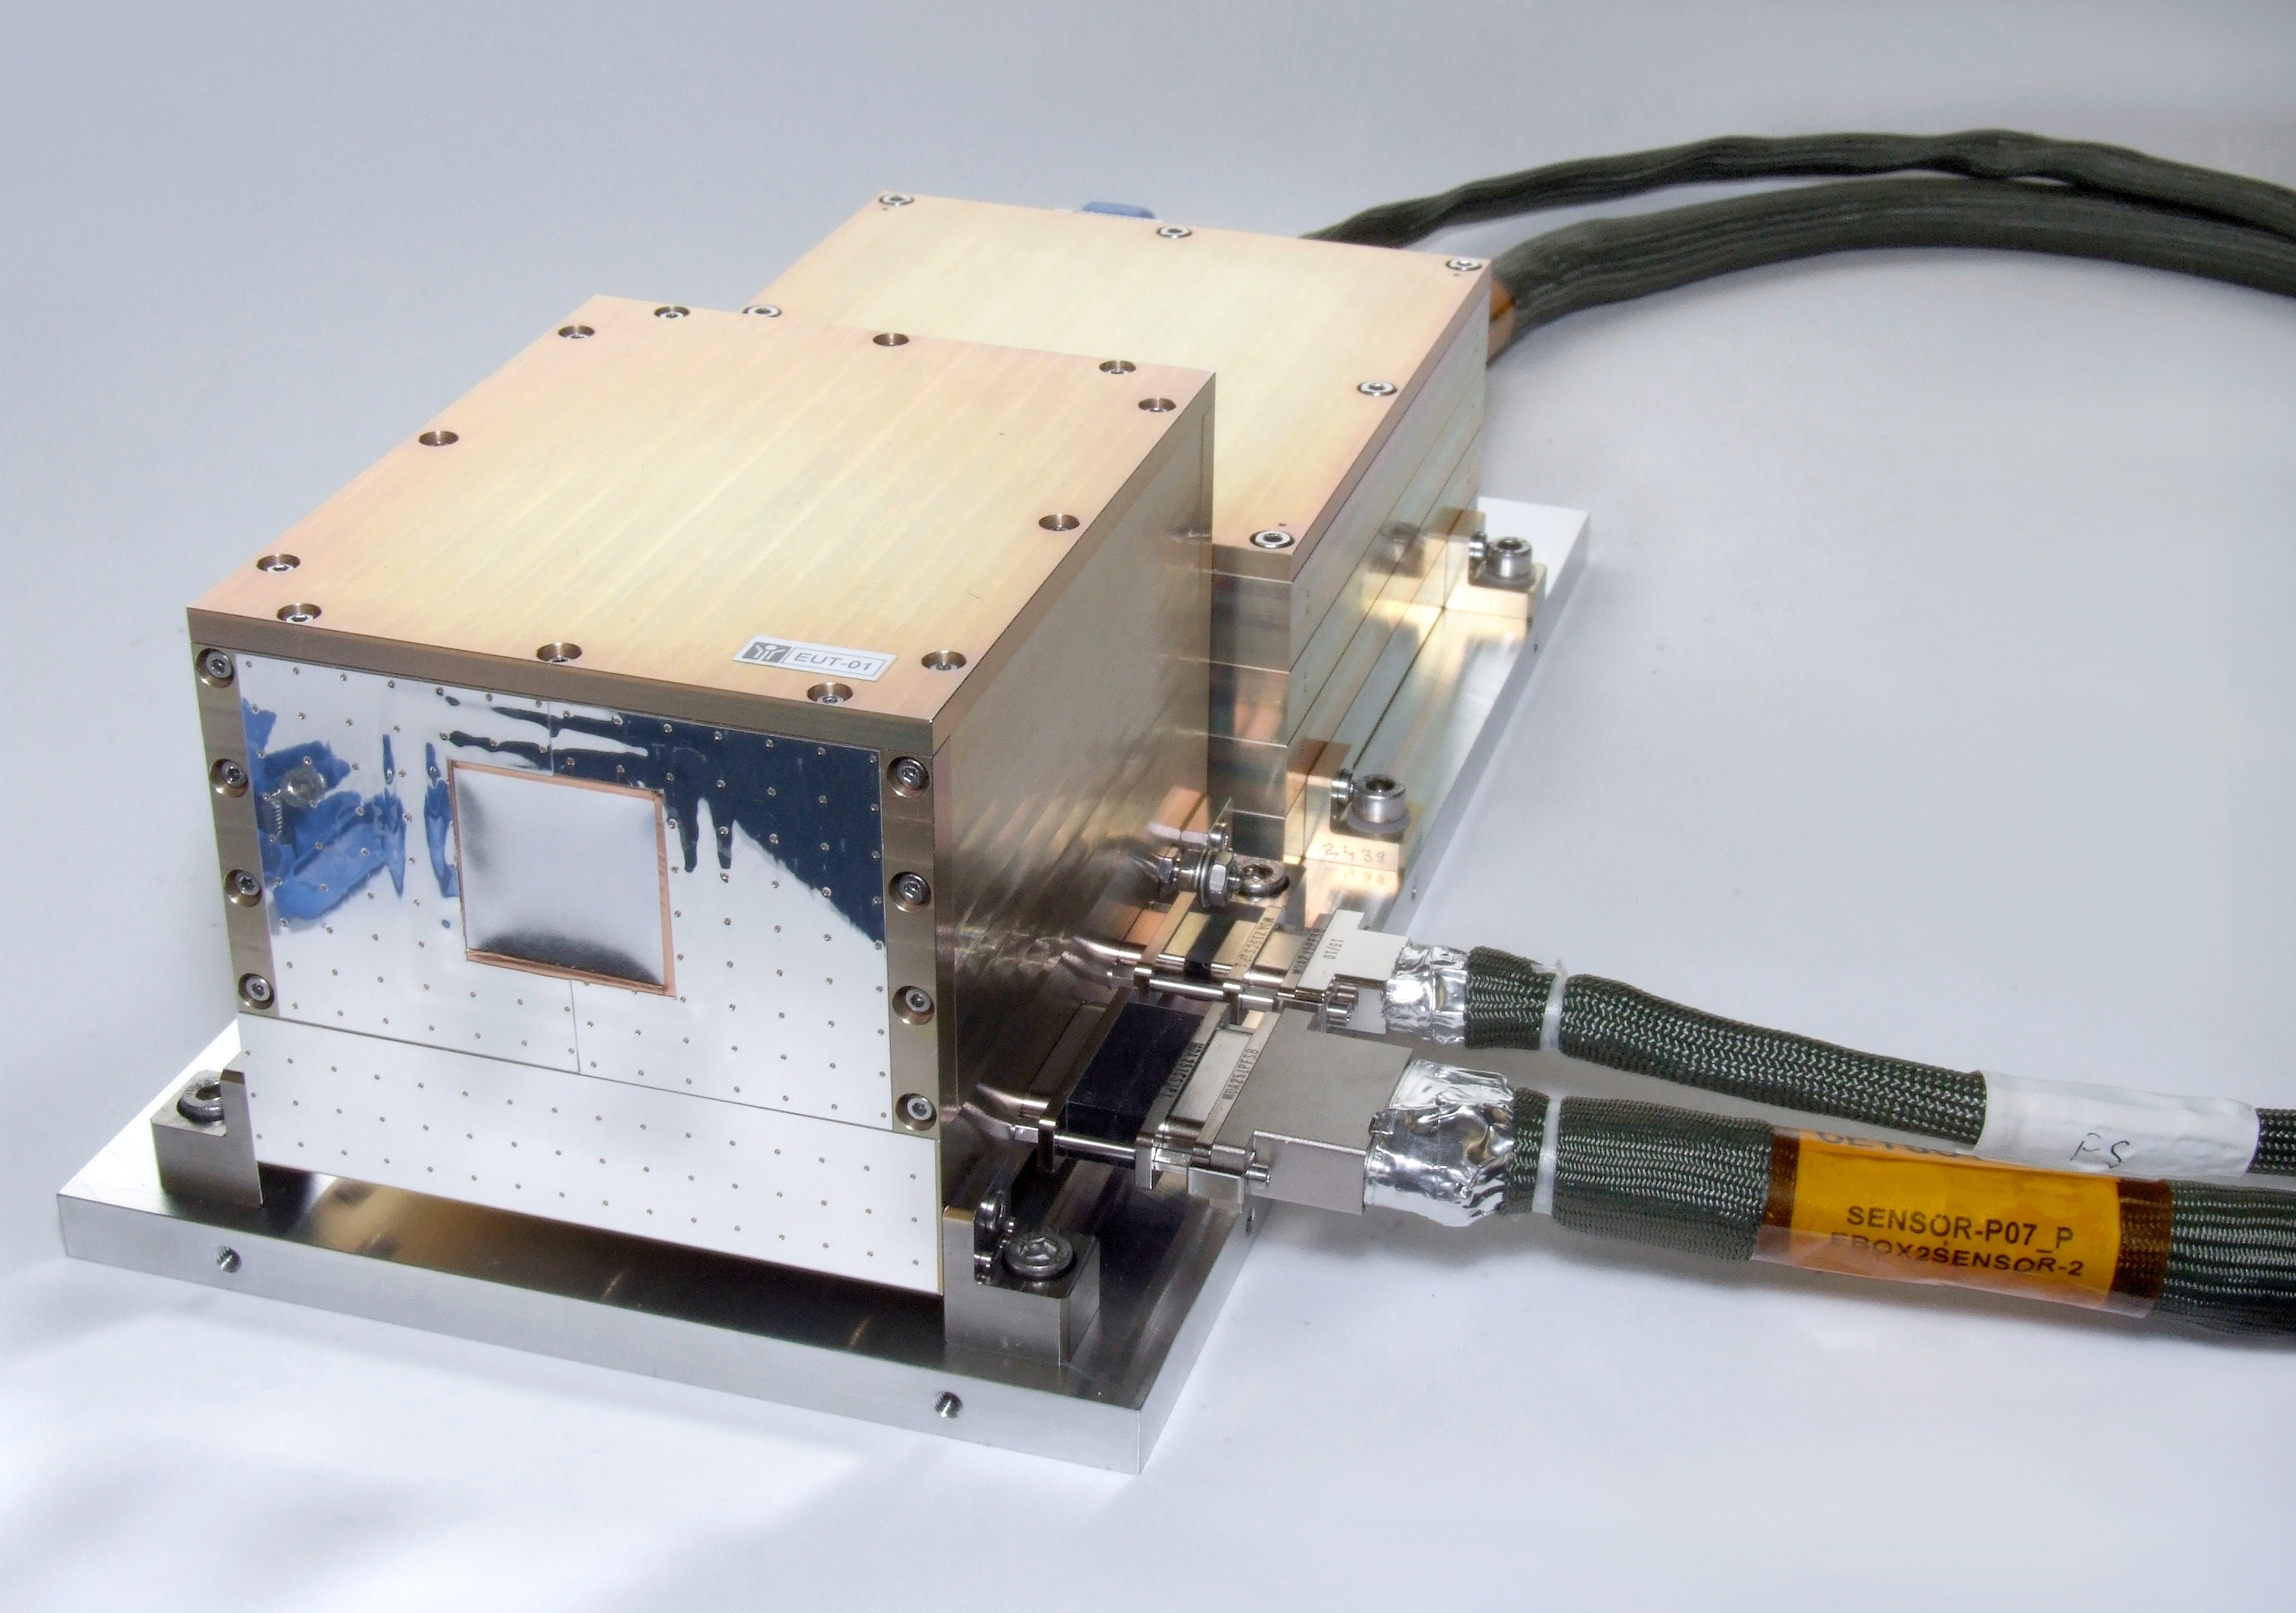
\includegraphics[width = 0.9\textwidth]{images/LND_2018-11-13.JPG}
    \caption[A Photograph of the \ac{LND}]{A photograph of the \ac{LND}, including the \ac{SH} in the front, \ac{EB} in the rear and 1-meters data and power harness that connects the \ac{SH} and \ac{EB}. The figure was adapted from \citet{Wimmer2020SSRv} and show the flight spare model of LND and was taken on 2018.11.23.}
    \label{Fig:LND_instrument}
\end{figure}


\begin{figure}[!htbp]
    \centering
    \includegraphics[width = 0.7\textwidth, height = 0.5 \textheight]{images/change4_lnd-c9_trigger-cones-colored.pdf}
    \caption[The inner structure of LND \ac{SH}]{A sketch of the inner structure of the \ac{LND} \ac{SH}. Ten 500 $\mu$m Si \acp{SSD} are assembled in order. The different colored regions indicate the \ac{FOV} of different measurement combinations. The figure was reproduced from \citet{Wimmer-2020-LND} and more details could be found in instrument paper.}
    \label{Fig:LND_sensor_head}
\end{figure}
Chang'E-4 is a robotic spacecraft mission of China exploring the lunar far-side surface, which is also the first human soft-landing missions on the lunar far-side surface \citep{Li2021SSRv}. The whole mission consists of a lander, a rover named Yutu-2 and a relay satellite named Queqiao which works in the lunar orbit and enables the communication between the lunar far-side surface and the ground. The mission was launched on December 8, 2018 and successfully landed on the Von K\`arm\`an crater near the south pole of Moon on January 3, 2019 \citep{Wu2019NatGe}. In order to cope with the significant temperature variations on the lunar surface, the rover, lander, and scientific payloads onboard enter a hibernation state during the approximately two-week-long lunar night. This mode helps to conserve energy power and to protect the detectors.  After the extended 'sleep' night, the instruments onboard are awakened by sunlight and start operating during the lunar daytime. The initial design life time of the mission was set at a minimum of one year. Obviously this target have been successfully surpassed and the scientific instruments onboard are continuing to perform impressive measurements.

As an integral part of the Chang'E-4 mission's international scientic payload, \ac{LND}\acused{LND} is designed by the Kiel University in Germany. An image of the flight spare model of \ac{LND} is displayed in Fig.~\ref{Fig:LND_instrument}. The initial design purpose of \ac{LND} is to measure the first active radiation dose rate and monitor the radiation environment caused by changed and neutral (neutrons and $\gamma$-ray) particles, as the preparation of future human exploration of the Moon and the solar system. 
Therefore, the main scientific objects of the \ac{LND}, as indicated in the instrument paper \citep{Wimmer-2020-LND}, are "Dosimetry for human exploration of the Moon" which is based on temporal variations of the dose rate and the \ac{LET} spectra, and "Contribution to the heliospheric science" which based on the measurement of charged particles.
% \begin{itemize}
%     \item \emph{Dosimetry for human exploration of the Moon}: \ac{LND} is designed to determine the temporal variations of the dose rate and the \ac{LET} spectra which will be used to derive the quality factor \textit{Q} which is a key factor to interprete the dosimetric data.
%     \item \emph{Contribution to the heliospheric science}: The particle fluxes and time series of the flux are measured on the far-side of the Moon. This unique measurement location provides valuable insights into the propagation of the particles in the heliosphere.
% \end{itemize}
Besides, \ac{LND} also has two technological demonstration objects which are "Determine the subsurface water content in the South-Pole Aitken Basin" and "Determine the FeO content in the South-Pole Aitken Basin" \citep{Wimmer-2020-LND}.

To achieve the aforementioned scientific objectives, \ac{LND} measures and provides the data products including up to 1-minute charged and neutral particle dose rate measured in Si, up to 1-minute cadence \ac{LET} spectra, 1-minute neutral particle deposition energy spectra, 10-minutes count rates of thermal neutrons and high time resolution (1-minutes, 10-minutes) charged particles flux and high energy resolution spectra including electrons and ions from proton to iron.

As of May 2023, \ac{LND} has been successfully working on the lunar far-side surface for more than 4 years, which corresponds to approximately 50 Lunar days since Jan 3, 2019. It has largely surpassed its designed lifetime.
One of the simplest way to check whether LND is working or not is to look up during the night and check the moon phase. If you can see a new moon or the moon is in the last/first quarter phase, it indicates that the moon is moving out of the earth's shadow and that the far-side surface of moon is facing the Sun, enabling the \ac{LND} work.

Based the the operations and experiment schedule established from the ground, \ac{LND} has been completely or partly (more than half a lunar day) switched off on the 6th, 44th, 45th lunar days since the start of the mission. As of the finalization of this thesis in May 2023, we have received 46 lunar days' data from January 2019 to the end of November 2022 which are stored on the servers of Kiel University. The data have officially been published in the Lunar and Planetary Data release system \footnote{\url{moon.bao.ac.cn}}, where currently the data is available until the end of December 2022. 
%you could find the data until December 2022. 
The alternative downloading options include \ac{NASA}'s Space Science Data Coordinated Archive and, \ac{ESA}'s archive ESDC (ESAC Science Data Center) which are still in building. The instrument will continue its operation on the lunar far side and we anticipate to receive can recive more intriguing data in the future with increasing solar activities.



\subsection{LND as Charged particle telescope}

\ac{LND} has a special designed sensor head that enables it to be used as a dosimeter, neutral telescope and charged particle telescope. Here, we put our focus on the charged particle telescope in this section and a brief introduction to the other two components are given in the next section for a comprehensive overview of LND's capability.

The flight spare model of \ac{LND} which is an exact replica of the flight model currently deployed on the moon is displayed in Fig.\ref{Fig:LND_instrument}. The instrument is composed of two seperate parts, the \ac{SH} in the front and the \ac{EB} at the rear. \ac{SH} and \ac{EB} are connected by a 1-meter cable which serves to provide power and transfer data. 
The \ac{SH} is comprised of ten Si \acs{SSD} of norminal 500 $\mu$m thickness. They are labeled from A to J and assembled in a charged-particle telescope configuration as illustrated in Fig.~\ref{Fig:LND_sensor_head}.

The structure of the telescope can be further divided into two parts. The upper half consists of four detectors (A, B, C, D) with A placed 80.5 mm away from B. The detector A is crucial for the function of \ac{LND} as charged particle telescope since only particles that trigger detector A will be counted. B/C/D are assembled as close in space as possible, with zero space between B and C and 0.5 mm between C and D, enabling the anti-coincidence measuremet in the inner C segement. Such a detector arrangement is similar to the Flight Radiation Environment Detector (FRED) \citep{moeller-etal-2013, moeller-etal-2013b}. The lower half consists of three detector pairs (E/F, G/H, I/J) and an Al-Gd-Al absorber. The detector pairs are closely packed together and the absorber is designed for the detection of thermal neutrons. 20 $\mu$m thick Gd foils are inserted into E/F and G/H, creating sandwich-like structures to detect thermal neutrons. This charged particle telescope is completed by the last detector pair I/J.

By measuring the energy depostion in different \acp{SSD} and using the dE/dX - E or dE/dX - dE/dX methods which depend on the primary energy of particles, LND can easily identify the energies and species of particles. 
The averaged energy loss of the charged particle along the travel path depends on the nuclear charge $Z_1$ (equal to atomic number) and the incident velocity $\nu$. 
Such a relationship could be expressed by the well-known Bethe-Bloch formula \citep{bethe-1930, bloch-1933}:

\begin{equation}
    \frac{\dd E}{\dd x} = - \frac{Z_1^2 e^4 n_e}{4 \pi \cdot \varepsilon_0^2 \beta^2 c^2 m_e} \cdot \left[ \ln\left(\frac{2 m_e  \beta^2 c^2}{{E_B}}\right) - \ln(1 - \beta^2) - \beta^2  \right], 
    \label{eq:BB}
  \end{equation}
where $c$ is the speed of light, $\beta = \nu/c$, $E_B$ is the ionization energy of the medium that particle pass, and $n_e$ is the electron density in the medium, $m_e$ is the electron mass, and constant $epsilon_0$ is the permittivity of free space. $E$ is the energy of the particle and $x$ is the travel length of the particle in the medium.

In the energy range that \ac{LND} covers, $ln(\beta^2)$ is nearly constant and slowly changes, hence the above function could be simplified as:
\begin{equation}
    E_A \propto \frac{Z_1^2 m_1}{E_{\mathrm tot}},
    \label{eq:BB2}
\end{equation}
The product of $E_A$ and $E_{tot}$ is proportional to the nuclear charge, $Z_1$ which equals to the atomic number and the mass of elements, $m_1$. These parameters depend on the particle species and allow for the determination of particle compositions. It is worth noting that \ac{LND} has the capability to discriminate between the isotopes of elements, such as helium-3 and helium-4, despite the limited resolution and larger uncertainty in the X-mas plot (Fig.~\ref{Fig:measurement_Xmas}, See Appendix \ref{chp:appendix_LND_He3_spectra})

%The nuclear charge $Z_1$ is equal to the number of protons in the nucleus, i.e. the atomic number $Z$ of the elements. Therefore, the telescope like \ac{LND} can not determine the particle charge state and we could not tell apart fully charged \ac{GCR} and singly charged \ac{ACR}. When traversing the front foil and \acp{SSD} of \ac{LND} sensor head, those partially charged particle will be ionized and stripped the electrons, becoming fully charged \citet{Swaczyna2017ApJ}.


Once the charged particle enter the sensor head of \ac{LND}, they can be further categorized into two groups: stopping particles and penetrating particles. Stopping particles have a primary energy range between $\sim$ 8 MeV/nuc and $\sim$ 35 MeV/nuc, stopping within any of the detectors B-I. Penetrating particles possess energy above this range and have the capability to penetrate through all the detectors. In Fig.~\ref{Fig:LND-Boehm-plot}, a plot generated by the large counting statistic \ac{Geant4} \citep{Agostinelli-2003} simulation illustrates how the stopping particles are seperated by using the $E_{tot} * E_A$ as the y-axis and $E_{tot} / E_A$ as the x-axis. The data points are simulated in \ac{Geant4} based on a carefully construced \ac{LND} instrument model. This model takes into account all the inner structures within the sensor head, including the \ac{PCB} next to the detector stacks and the outer shell of the sensor head. However, we must note that a completed model including the surrounding material of \ac{LND} is unavaiable since we lack the structure information of the Chang\'E-4 lander.
A screenshot of the \ac{LND} model is provided in the appendix \ref{chp:LNDsimulation}. 

Penetrating particles have a primary energy above approximately 35 MeV/nuc, and as the name suggested, can penetrate through detectors A to I and stop in J or continue to penetrate J with more energy. The majority of the penetrating particles are fully penetrating particles, which means we can not directly measure their total energy. \acp{MIP} are among the fully penetrating particles that have extremely large initial energy from hundreds MeV to GeV but only deposit a minimal amount of energy in the detector stacks.
Since the total energy of particles is unavaiable, it is not possible to create a plot similar to Fig.~\ref{Fig:LND-Boehm-plot}. Instead, we change the formula of x-axis and y-axis to $E_I/E_A$ and $dE$ respectively. The $E_I$ is the energy deposit in the last detector I. The $dE$ is the energy deposition summed from the B, C, and D.

Notably the incident direction of the particle i.e. whether they come from above or beneath the detector, could be inferred from the penetrating data. Typically, for the particle incident from above, the ratio $E_I/E_A$ tends to be larger than 1 and while for particles entering from beneath, this value tends to be less than 1. 
By analyzing the distributions and patterns in the histogram, we can identify the albedo protons from the 2-D histogram of penetrating particles, corresponding to columns 248 - 264 in the Xmas plot (Fig.~\ref{Fig:measurement_Xmas}).
The detailed understanding of the derivations and analysis of albedo protons could be inferred from Section. ~\ref{chp:LND_GCR_albedo}


\begin{figure}
    \centering
    \includegraphics[width=0.8\textwidth]{images/LND_Boehm_plot_isotropic_on_top_of_A_annotated.png}
    \caption[LND Boehm plot of stopping particles based on the simulated data]{The different particle species are well discriminated in this LND Boehm plot which is a scatter plot of the \ac{LND} simulation data generated by the \ac{Geant4} tools \citep{Agostinelli-2003}. During the simulation, an isotropic source is positioned above detector A.}
    \label{Fig:LND-Boehm-plot}
\end{figure}


\subsection{LND as dosimeter and neutral telescope}

\ac{LND} measures the \ac{TID} in the inner B segment utilizing the energy deposition and corresponding energy spectrum. The inner segment of C, which is surrouded by the B, D and C outer segment and in anti-coincidence with all other detector segments, is used to measure the neutral dose rate caused by both fast neutrons and $\gamma$-rays. The above two measurements are the primary data products of \ac{LND}. \ac{TID} and dose in C play important roles in assessing the radiation environment on the lunar surface. 

\ac{LND} employs the E/F, G/H pairs which clamp a Gd-foil, to measure the thermal neutron flux. The Gd-foil has a large cross section for thermal neutrons, resulting in an increased possibility of interaction with those neutrons. In the calibration experiment, \ac{LND} successfully measured neutrons by calculating the energy spectrum discrepancy between E (G) and F (H) for neutrons coming from the front (back) \citet{Wimmer2020SSRv}.
However, in real measurements, the quality of the thermal neutron data is unexpectedly low due to various factors. The most prominent factors is the neutron background emitted from the \ac{RTG} and the \ac{RHU}. These radioactive sources generate heat to protect the lander and payload from the frozen night. But they also contribute largerly on the neutron background \citep{Zhang2020SciAdv}. Unfortunately, the direct measurement of the radiaion sources had never been done, and only an experimental and empirical estimation of the contamination from the background on the data were conducted by \citet{Hou2020-LNDbackground}. Based on data from laboratory experiements and Monte-carlo simulations, \citet{Hou2020-LNDbackground} confirmed the non-negligible background interference and firstly estimated the dose rate background. 

Another factor that might affect the neutron measurements is the unanticipated noise increase in these detectors. Similar to the noise issue occured in other channels, channels F2, G2 and H1 have also been troubled by an increased noise level (further discussed in Section \ref{chp:LND_GCR_albedo}). The single detector counter rates increase from $10^3$ count/min to $10^6$ count/min and energy spectra of noise channels indicate that the dominant energy is below 300 keV.
The high energy noise obscure the x-ray line at 43 keV and electron lines at 71 keV, 131 keV, and 173 keV which are used to determine the thermal neutrons flux, and make it more challenging to derive the accurate thermal neutron flux of lower intensity.
Furthermore, enhanced number of noise in those thermal neutron channels cause serious dead time issues on the data product neutron dose in C. This is because neutron measurements share the same counter buffer. The dose in C is the primary objective of \ac{LND}. In order to mitigate the dead time issue, we raise the corresponding threshold of noise detectors to few hundreds keV (depending on the noise level of each detector), resulting in the loss of the thermal neutrons data.


The remain data products related to the radiation are the \ac{LET} spectra. \ac{LND} provides three types of \ac{LET} spectra including \ac{LET} $ABC\bar{I}$, $\bar{A}BIJ$ and $ABIJ$. Those \ac{LET} spectra can be used to derived the quality factor (Q), which multiplies the absorbed dose rate to obtain the dose equivalent.
Of note is that geometry factors of these \ac{LET} spectra are also affected by the configuration changes. We provide the changes of geometry factors in the appendix of chapter \ref{chp:LND_GCR_albedo}.
%More details of the data products can be found in the instrument paper \citet{Wimmer2020SSRv}.

The first scientific result of \ac{LND} regarding the radiation environment on the lunar surface are reported in \citep{Zhang-2020-LND-firstresults}. These initial findings present the \ac{TID}, neutron dose and \ac{LET} spectra of the first two lunar days. This represents the first ever dynamic measurements of the radiation variation on the lunar surface. The averaged total absorbed dose rate in silicon is about 13.59$\pm$1.01 $\mu$Gy/hour. Amongst this total dose rate, the contribution from neutral particles is estimated to be $3.10 \pm 0.43 \mu$Gy/hour. These values are consistent with the measurements from the \ac{CRaTER} on \ac{LRO}.



\subsection{Primary data products: Xmas plots}
\label{sec:xmas}

\begin{figure}
    \centering
    \includegraphics[width =0.8\textheight, height = 0.6\textheight, angle = 90]{images/xmas-2019-01-03To2022-11-29.png}
    \caption[\ac{LND} Xmas plot from measurements]{The completed Xmas plot (274 $\times$ 64) of \ac{LND} based on the measurements between 2019.1.3 and 2022.11.29. All the data products could be found in this matrix, including neutrals, \ac{LET} spectra, \ac{TID}, stopping and penetrating charged particles, including electrons, protons, helium nuclei and heavy ions. The corresponding simulation version can be found in \citep{Wimmer2020SSRv}}
    \label{Fig:measurement_Xmas}
\end{figure}

Fig.~\ref{Fig:measurement_Xmas} is the so-called "Xmas plot" \footnote{It was the front cover of the Xmas card of IEAP group in 2017. Hence we named it Xmas plot} of the \ac{LND}.The Xmas plot is an image of \ac{LND}'s memory space shaped in a 274 $\times$ 64 matrix, where each pixel in the Xmas plot servers as a counter. In principle all data products are extracted from this matrix. 
When \ac{LND} detects the deposited energy in detectors of an effective signal, the control units will calculate onboard the appropriate position in the Xmas plot and increment the corresponding counter. 

Unlike the simulated plot in \citep{Wimmer2020SSRv}, here we showcase an Xmas plot from the actual measurements between 2019.1.3 to 2022.11.29, encompassing all the data accumulated since the first lunar day observed by \ac{LND}. The green rows are the memory space that will not be transmitted to the ground, in order to save the telemetry bandwidth. 
For a more detailed explanation of the format of the Xmas plot, I recommend \citep{Wimmer2020SSRv}.

%The major different compared with the Xmas plot in \citep{Wimmer2020SSRv} is that LND measure not only the particle incident from above but also the albedo particles moving upward, while in the simulation, we did add the albedo component. It is obvious that in the penetrating panel of Xmas plot,  a higher than backgrond branch strech from middle to the left side. This branch represents the protons moving upward with enough energy fully penetrating all the detectors as well as the extra shielding from the lander structure. More details of how to derive albedo proton flux are given in Section.~\ref{sec:albedo_proton}.

\subsection{Configuration changes of LND}

It is important to highlight that several configuration changes have been implemented after \ac{LND} was delivered and launched. Those configuration changes are reflected in 14 extra commands, which are uploaded to the control unit of \ac{LND} every morning of lunar day, fixing software issues and malfunction issues. One of the software issues arises from errors in the software pipeline where the control unit use wrong channels to determine particle energies. Another one is due to the mistakes we made in simulations when designing data products, causing location of the \ac{dps} boxes shift in the X-mas plot which is a matrix storing \ac{LND} data products (See below and \citet{Wimmer-2020-LND} for more details about the X-mas plot). Neverthless, the impact of the second problem on the data products is minor. 

The significant changes of the data products are mainly caused by raising the threshold of noise channels and by removing the A2 channel in the level 3 trigger logic. A2 represents the outer segement of the front detector A (see Appendix in Sec.~\ref{chp:LND_GCR_albedo} for more details of the changes). These changes are motivated by high observed noise levels in detectors A, G, H, I and J which appeared coincidentally with the malfunction of the front lid. The front lid of \ac{LND} is a part of the lander and is designed to protect the fragile detectors inside the \ac{SH}. The lid is opened up to allow unobstructed measurements of the particles during lunar days, and is closed immediately after the instrument is switched off, protecting the detectors from the extreme temperature dercrease on the lunar surface and the lunar night. However, on the 3rd and 4th lunar day, \ac{LND} was switched off for a short period during working time but the lid was left open. Though temperature on the lunar surface increased as the Sun rose, \ac{LND} and its detectors kept losing heat. Hence the temperature of the \ac{SH} dropped drastically, resulting in irreversible deformation of carriers and the attached detectors, particularly the detectors A and I/J in the front side and the bottom side. Consequently, the lower energy noise ($\sim$ 10 - 200 keV) experienced a significant increase.

By implemmenting the aforementioned changes, we have sucessfully reduced the noise level and mitigated its impact on the primary data products such as \ac{LET} spectra. However, it is worth noting that these changes still resulted in significant consequences for several data products. For instance, we partly lose the measurement of \acp{MIP} after the increment of the threshold of I detector; the geometry factors of two \ac{LET} spectra and penetrating particle are reduced dramatically after disabling the A2 channel, which plays a key role in \ac{LND}'s measurement logic. For a better understanding of the configuration changes and their impact on the data products, please refer to the appendix of chapter \ref{chp:LND_GCR_albedo}.
The corresponding changes of the original code in the LND data processing pipeline is given in the appendix ~\ref{chp:appendix_LND_data_process_pipeline}.

\section{Solar orbiter and High energy telescope}

Successfully launched on Feb 10, 2020, \ac{SolO} mission \citep{Mueller-2020-SolO} is an international mission cooperated between \ac{ESA} and \ac{NASA} with the aim to understand the Sun and how it controls the helisphere. As indicated in the mission paper, the following scientific questions will be answered and further studied: (a). What drives the solar wind and where dose the coronal magnetic field originate from? (b). How do solar transients drive heliospheric variability? (c). How do solar eruptions produce the energetic particle radiation that fills the heliosphere? (d). How does the solar dynamo work and drive connections between the Sun and the heliosphere?

%After finishing the cuise phase which started at June 14, 2020, \ac{SolO} has been operating in the nominla mission phase since Nov 26, 2021 as scheduled.

\ac{SolO} has an elliptic helioscentric orbit with the closest perihelion of 0.29 AU (about 42$\times10^6$ km). Using several gravity assist maneuvers during the Venus flybys and the Earth flybys, the orbit of \ac{SolO} will gradually tilt away from the ecliptic plane and in the end can be 24 degrees above the Sun's equator. As of May 2023 \ac{SolO} is still following an elliptical orbit circling the sun, with a maximum solar latitude of 8.66 degrees. \ac{SolO} has finished 5 perihelions with a closest distance of 0.292 AU on Sep 3, 2022, and has started its 6th orbit, moving away the Sun. Benefiting from the unique position of \ac{SolO} during this trip, the multiple scientific instruments onboard the \ac{SolO} could further advanced our understanding of the Sun and its effects on the heliosphere.
%Three time Venus flyby happened on Dec 27, 2020,  Aug 9, 2021 and Sep 4, 2022. The Earth GAM happend on Now 27, 2021.
%The above mentioned solo tragjectory information is taken from the Solar orbiter Consolidated Report on Mission analysis \footnotes{\url{https://issues.cosmos.esa.int/solarorbiterwiki/display/SOSP/Trajectory+Overview+-+10+February+2020+Launch}}

%in the relative field for instance the questions regarding solar coronal, solar magnetic field, solar wind, \ac{SEP}.
The \ac{EPD} \citep{RodriguezPacheco-2019-EPD} is part of the scientific payload onboard \ac{SolO}, measuring energetic particles over a large scale from few kev to GeV. The spectra, composition, time variations and directional distributions could be obtained and derived.
\ac{EPD} is comprises of four different sensors, the \ac{SIS}, the \ac{STEP}, the \ac{EPT} and the \ac{HET}. 
\ac{SIS} is a time-of-flight mass spectrometer that measures ion composition from $\sim$ 0.1 - few MeV nucleon$^{-1}$. \ac{STEP} measures electrons and ions with lower energies between 4 keV and 80 keV. The special design of \ac{STEP} allows it to have high pitch-angle resolution.
\ac{EPT} and \ac{HET} share the same electronics and they are composed of two identical sensor units that are assembled perpendicularly on \ac{SolO}. This configuration enables detection of the particle incident from four different directions. \ac{EPT} is designed to measure medium-energy electrons and ions within the energy range of 25 keV to 400 keV ($\sim$ 6 MeV for protons), while \ac{HET} completes the higher energy end, measuring electrons from 300 keV to 30 MeV and ions from 6.8 Mev/nuc to $\sim$ 100 MeV/nuc in the nominal data products. Notably, the penetrating data products of \ac{HET} could extend the energy coverage of \ac{HET} up to $\sim$ GeV/nuc \citep{Elftmann-2020-PhD}.
The completed energy coverage of those four instruments for different particle species are given in Fig.~\ref{Fig:EPD-energy-coverage}.
In this section, we provide a brief introduction of \ac{HET}, which is the focus of the study in Section \ref{chp:ACR_Helium}. Further more detailed information on the other components can be found in the instrument paper \citep{RodriguezPacheco-2019-EPD} and the first years overview paper from \citet{Wimmer2021AA}.


\begin{figure}
    \centering
    \includegraphics[width = \textwidth]{images/EPD_coverage.png}
    \caption[The energy coverage of \ac{EPD} instruments]{The energy coverage of different \ac{EPD} instruments for different particle species. This figure is an updated energy coverage plot made by \citep{JohanPhd2020}, based on the similar plot from \citep{RodriguezPacheco-2019-EPD}. The HET measurements are split into stopping and penetrating parts and the later one can largely extend \ac{HET}'s capability \citep{Elftmann-2020-PhD}.}
    \label{Fig:EPD-energy-coverage}
\end{figure}  

\subsection{High energy telescope}

\begin{figure}
    \centering
    \includegraphics[width = \textwidth]{images/het.png}
    \caption[The \ac{HET} sensor head]{The cross profile of the \ac{HET} sensor head. The detector names are labeled. Figure is reproduced from \citet{RodriguezPacheco-2019-EPD}.}
    \label{fig:HET-sensor-head}
\end{figure}

\ac{HET} is a double-ended telescope. The cross profile of the \ac{HET} sensor head is depicted in Fig.~\ref{fig:HET-sensor-head}. The sensor head of \ac{HET} consists of four 300 $\mu$m silicon \ac{SSD} stacks, with two in each side (A1, B1 in the front side and A2, B2 in the back side), and a 2-cm thickness \ac{BGO} ($Bi_{4}Ge_{3}O_{12}$) scintillator which is named as detector C in the center. The sensor head setup is similar to the configuration of the \ac{RAD}, another instrument developed by Kiel Univeristy, which is currently operating on the Martion surface.  

\ac{HET} uses the $\mathrm{dE/dX - E}$ technique to discriminate different particle species of different energy. This method is the same as the measurement principle of \ac{LND} that has been well explained before. The particle species that \ac{LND} can discriminate include electrons, protons, helium nucleus, and all heavy ions such as carbon, nitrogen, oxygen, and iron.  

Once the charged particle incident and penetrate the A detector (A1 or A2), they can be split into stopping particles and penetrating particles, depending on their energy and whether they stop in detector B/C. As given in Table 22 of \citet{RodriguezPacheco-2019-EPD}, the corresponding nominal data products are ABnC, which is corresponding to particles stopping in B with energy of 6.5 - 9.5 Me/nuc, ABC which register particles stopping in C with energy range of $\sim$10 - $\sim$ 100 MeV/nuc, and penetrating detector C with energy above 100 MeV/nuc up to infinity. 

%For the penetrating particle, their primary energy can be estimated based on the energy loss on the detector and the \ac{Geant4} simulation. The aforementioned nominal data products of HET contribute to the study of \ac{SEP}, \ac{ACR} and \ac{GCR}.


In addition to the nominal charged particle data products, it is important to emphasize the significant contribution of housekeeping data in our studies.
The housekeeping data are \ac{EPD} sensor produced instrumental data. They have the highest priority for downlink to the Earth and are used to monitor the instrument status and health. Although the housekeeping data are not designed for scientific purpose, they still provide valuable insight into the instrument performance and their contributions to the scientific studies is impressive \citep{Wimmer2021AA}.


Such a housekeeping data is the single detector counter which register signals in the \ac{BGO} scintillator crystal, this is the C detector. This counter does not require any coincidence condition and respond to particles from all directions and types. The sole requirement is that the deposited energy exceeds the threshold of the C detector. Due to its larger geometry factor, this counter exhibits better counting statistics and can be used to detect small disturbance in the \ac{GCR} background. For example \citet{Forstner-2021-SolO} use this counter to study a \ac{FD} with an ampliude of 3\% when a \ac{CME} passed \ac{SolO} on 19 April 2020. In addition, \citet{Allen2021AA_venus} found an $\sim$ 5\% drop in the count rates during the first Venus flyby. This drop is due to the planet body blockage on the \ac{FOV} of \ac{HET}.

Similar to the single detector count rate, we also utilize the L2 counters named \textit{any(a1, b1)} or \textit{any(a2,b2)} to determine the periods of \acp{SEP}. The counters sum up every signal that triggers detectors A1 (A2) and B1 (B2) in the sensor head, regardless of the primary energy and the particle species. \acp{GCR} which are slowly varying are the dominant particles in the background of this counter. Therefore, a temporal increase indicates an incoming of \ac{SEP} event. These data products exhibit better counting statistics than the nominal science data products which are designed to derive the flux. Additionally, \textit{any(a1, b1)} or \textit{any(a2,b2)} are more sensitive to lower energy particles from \acp{SEP}, as they have a lower energy threshold of $\sim$ 50 keV compared to the C counter \citep{Elftmann-2020-PhD}. The counters can detect electrons and ions with energy below 1 MeV. As a result, those two counters are particularly useful in determining the start and end time of the \ac{SEP} events, no matter what particles trigger them. In Section~\ref{chp:ACR_Helium}, where we are interested in \acp{ACR}, we remove \ac{SEP} time periods determined by this method based on the \textit{any(a1,b1)} counter to enable an accurate \ac{ACR} measurement.

For more details on the inner structure and parameters of the \ac{HET}, as well as the most update status of \ac{HET}, one could refer to \citet{RodriguezPacheco-2019-EPD, Wimmer2021AA,Elftmann-2020-PhD}.



\chapter{Solar energetic particles (SEPs) event on the lunar far-side surface}
\label{chp:LND_SEP}


The Chang'E-4 mission, initiated in 2019, coincided with a period of solar minimum characterized by a scarcity of \ac{SEP} events. However, as sun stepping into the increase phase of new \ac{SC} and becoming more active than the solar minimum, solar activity has intensified, and consequencely, a growing number of \acs{SEP}, including prolonged-duration and high-intensity one, have been observed to reach the lunar surface and have been detected by the \ac{LND} on the lunar far-side surface. For example, Guo et al. (2023) recently reported the first \ac{GLE} of \ac{SC} 25, which were concurrently detected by instruments deployed on the Moon, Earth, Mars and also by \ac{SolO} as well as \ac{PSP} [citation of other studies]. It is noteworthy that \ac{LND} was switched on during the the decay phase of this events, hence missed the onset phase of the event. Even so, it still improves our understanding of potential radiaton risk that caused by those extreme \ac{SEP} events on the planetary surface.
In the appendix section of this thesis, a comprehensive list of \ac{SEP} events detected by the \ac{LND} on the lunar far-side surface between 2019 and 2023 is provided, further emphsizing on \ac{LND}'s contribution to the study of \acs{SEP}.


The \ac{SEP} event happened on May 6, 2019 is the first \ac{SEP} event that have was detected on the lunar surface in the past decade, according to our knowledge. 
This \ac{SEP} event is associated with an M-class flare originating from solar active region (AR12470) which is located on the eastern hemisphere and is more than 110 degrees away from the Earth's magnetic footpoint on the solar surface. The remote-sensing observations conducted by the \ac{SOHO}/\ac{LASCO} and \ac{STEREO} revealed the presence of a slow, narrow, and westward moving \ac{CME}. 
Though those \acs{SEP} cause negligible radiation dose due to its weak intensity and lower peak energy, it is still an interesting event and worth studying due to the following two reasons.
The primary objective of this study is to utilize the first \ac{SEP} event observed by \ac{LND} to validate the data products produced during \ac{SEP} occurrences and assess the instrument's performance under such conditions. By cross calibrating the proton measurements between \ac{LND} and other already existed particle instruments at the first lagrange point, specifically the \ac{EPHIN} onboard \ac{SOHO} and \ac{ACE}/\ac{EPAM}, we conclude that \ac{LND} provide reliable solar energetic proton measurement with high time resolution of one minute.
%For sure LND is outside of the mangetosphere, but still that is one of the thing worth to look at. How the SEP propogarting across the magnetosphere and arrive the magnetosphere tails.
Additionally, we aim to investigate the extensive spatial distribution of this \ac{SEP}. Several mechanisms could be invovled in the process of the particle traversal across considerable distance in the so-call wide spread \acs{SEP}. Combined the in-site and remote-sensing measurement, we try to found out what kind release and propagation mechanism are involved in this event.

The following article is reproduced from \textcite{Xu2020ApJ} by permission of the AAS:\\

\noindent\pubcite{Xu2020ApJ}\\
\strut\hfill Own contribution: 80\%

\newpage
\newcounter{includepdfpageAPJLTwenty}

\addtocounter{section}{1}
\setcounter{section}{1} 
% \phantomsection
% \addcontentsline{toc}{section}{\arabic{chapter}.\arabic{section} First Solar Energetic Particles Measured on the Lunar Far-side(Publication ApJ Letter 2020)}
%
\phantomsection
\addcontentsline{toc}{section}{\arabic{chapter}.\arabic{section} Introduction}
\label{sec:paper_xu2020}
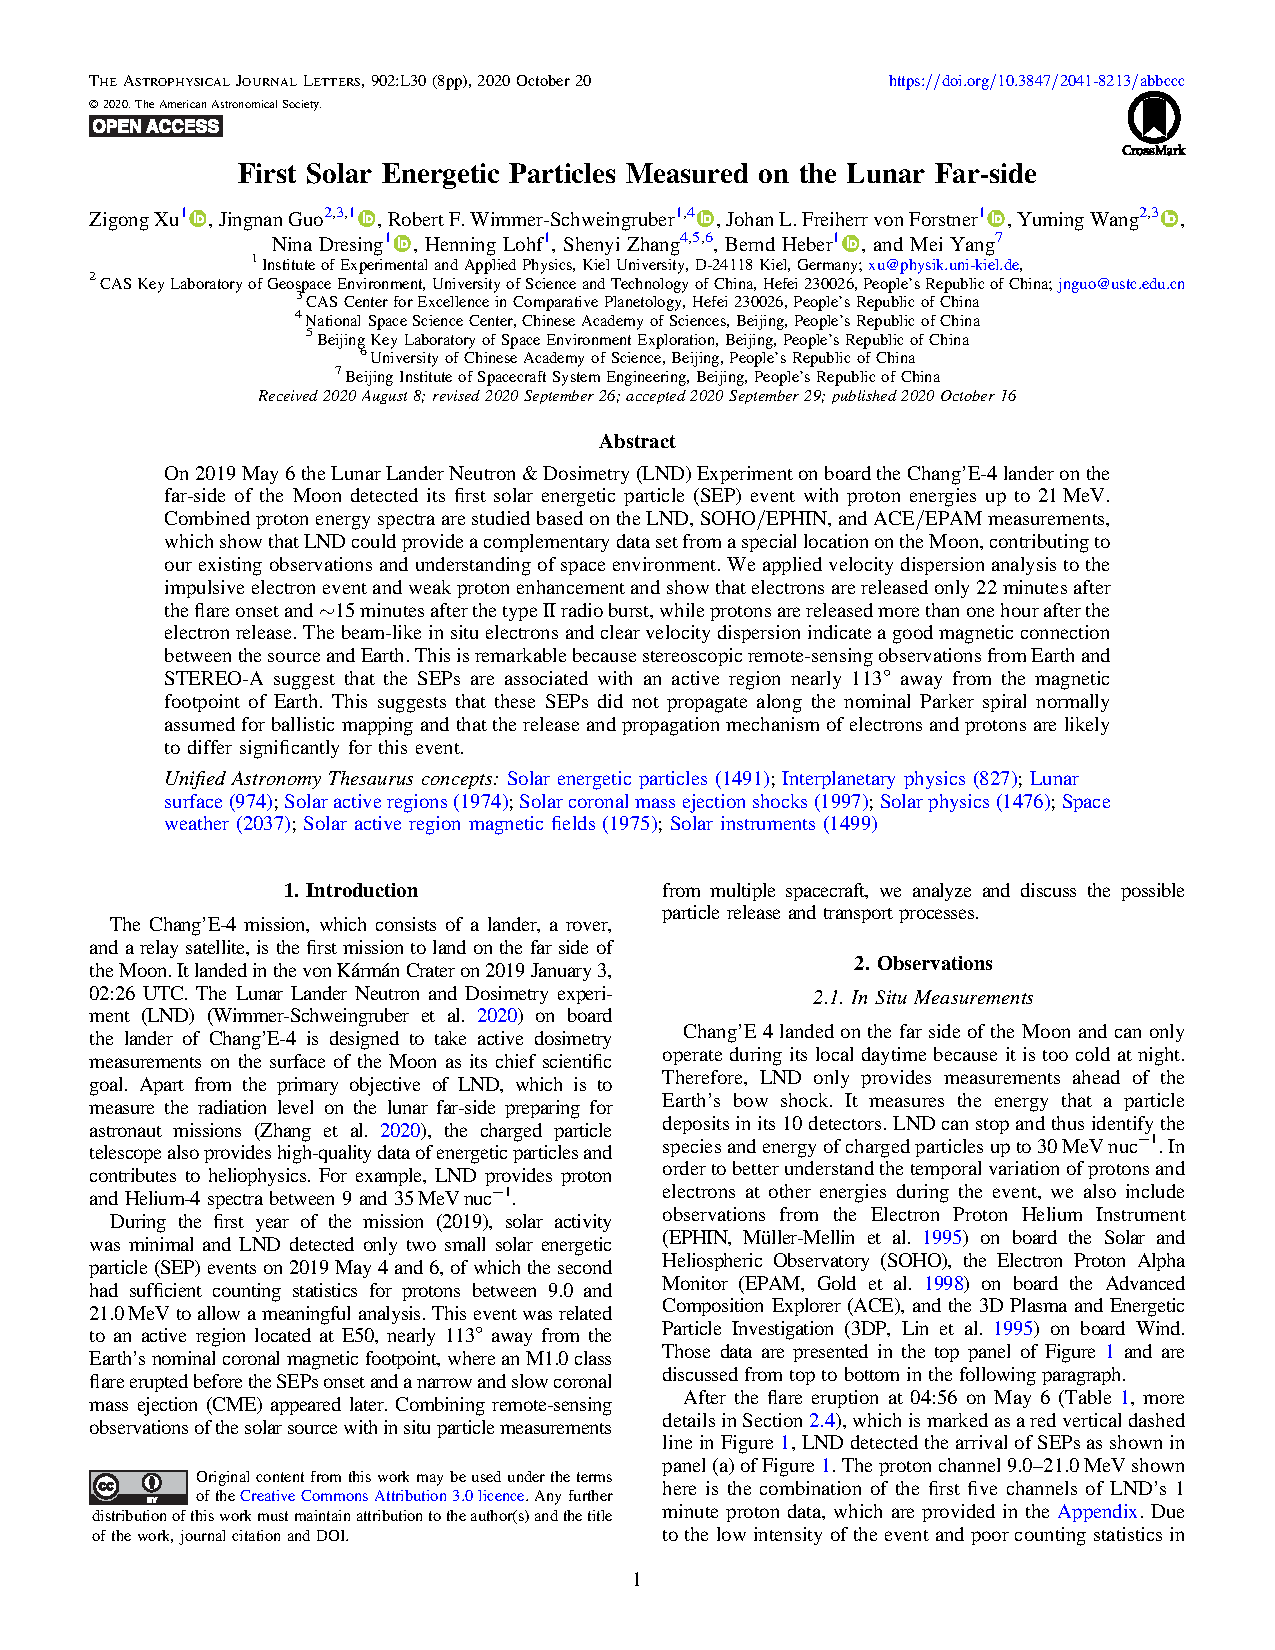
\includepdf[pages={1}, link, linkname=paper_xu2020, scale=.9, pagecommand={\refstepcounter{includepdfpageAPJLTwenty}\label{paper_xu2020.\theincludepdfpageAPJLTwenty}}]{publications/Xu_et_al_2020_ApJL.pdf}
%
\addtocounter{section}{1} 
\phantomsection
\addcontentsline{toc}{section}{\arabic{chapter}.\arabic{section} Observations}
\includepdf[pages={2-4}, link, linkname=paper_xu2020, scale=.9, pagecommand={\refstepcounter{includepdfpageAPJLTwenty}\label{paper_xu2020.\theincludepdfpageAPJLTwenty}}]{publications/Xu_et_al_2020_ApJL.pdf}
%
\addtocounter{section}{1} 
\phantomsection
\addcontentsline{toc}{section}{\arabic{chapter}.\arabic{section} Summary and Discussion}
\includepdf[pages={5-6}, link, linkname=paper_xu2020, scale=.9, pagecommand={\refstepcounter{includepdfpageAPJLTwenty}\label{paper_xu2020.\theincludepdfpageAPJLTwenty}}]{publications/Xu_et_al_2020_ApJL.pdf}
%
\addtocounter{section}{1} 
\phantomsection
\addcontentsline{toc}{section}{\arabic{chapter}.\arabic{section} Appendix}
\includepdf[pages={7}, link, linkname=paper_xu2020, scale=.9, pagecommand={\refstepcounter{includepdfpageAPJLTwenty}\label{paper_xu2020.\theincludepdfpageAPJLTwenty}}]{publications/Xu_et_al_2020_ApJL.pdf}
%
\addtocounter{section}{1} 
\phantomsection
\addcontentsline{toc}{section}{\arabic{chapter}.\arabic{section} References}
\includepdf[pages={8}, link, linkname=paper_xu2020, scale=.9, pagecommand={\refstepcounter{includepdfpageAPJLTwenty}\label{paper_xu2020.\theincludepdfpageAPJLTwenty}}]{publications/Xu_et_al_2020_ApJL.pdf}


\chapter{The quiet time GCR protons and albedo protons measured on the lunar far-side surface}
\label{chp:LND_GCR_albedo}

(This this the start page of the LND GCR and albedo protons)


The moon is expose to the deep space. 


GCE from outside of Solar system, accelerated by the shock wave.


From 2019.1 to 2020.7, apart from the SEP event that we studied in the last chapter, no SEPs arrived on the lunar surface during this period, 
hence it is a good opportunity to study the galactic cosmic rays (GCRs) and the albedo protons.




GCR dominate the quite time
LND start from solar minimum, good opptunity to study the GCR

Beside,


We reproduced the following article from the published paper \citep{xu2020} under the CC BY 4.0 license as following and in the end of this , we give the configuration changes since LND landed and launched. 

The following articles is reproduced from the published paper \citep{xu2022} under the CC BY 4.0 license.






The following article is reproduced from \textcite{Xu2022FrASS}, which is an open-access article reproducted under the terms of 
the CC-BY license. The supplement material including the configuration changes of LND up to now and the data we used in the main content is attached afterward. 
\\

\noindent\pubcite{Xu2022FrASS}\\
\strut\hfill Own contribution: 90\%

\newpage
\newcounter{includepdfpageFrontierTwentyTwo}

\addtocounter{section}{1}
\setcounter{subsection}{1} 
\phantomsection
\addcontentsline{toc}{section}{\arabic{chapter}.\arabic{section}. Primary and albedo protons detected by the Lunar Lander Neutron and Dosimetry experiment on the lunar farside(Publication Frontier in Astronomy and Space Sciences 2022)}
%
\phantomsection
\addcontentsline{toc}{subsection}{\arabic{chapter}.\arabic{section}.\arabic{subsection} Introduction}
\label{sec:paper_xu2022}
\includepdf[pages={1-3}, link, linkname=paper_xu2022, scale=.9, pagecommand={\refstepcounter{includepdfpageFrontierTwentyTwo}\label{paper_xu2022.\theincludepdfpageFrontierTwentyTwo}}]{publications/Xu_et_al_2022_Frontier.pdf}
%
\addtocounter{subsection}{1} 
\phantomsection
\addcontentsline{toc}{subsection}{\arabic{chapter}.\arabic{section}.\arabic{subsection} Preparation of LND data}
\includepdf[pages={4-8}, link, linkname=paper_xu2022, scale=.9, pagecommand={\refstepcounter{includepdfpageFrontierTwentyTwo}\label{paper_xu2022.\theincludepdfpageFrontierTwentyTwo}}]{publications/Xu_et_al_2022_Frontier.pdf}
%
\addtocounter{subsection}{1} 
\phantomsection
\addcontentsline{toc}{subsection}{\arabic{chapter}.\arabic{section}.\arabic{subsection} Measurements and comparison with model}
\includepdf[pages={9-11}, link, linkname=paper_xu2022, scale=.9, pagecommand={\refstepcounter{includepdfpageFrontierTwentyTwo}\label{paper_xu2022.\theincludepdfpageFrontierTwentyTwo}}]{publications/Xu_et_al_2022_Frontier.pdf}
%
\addtocounter{subsection}{1} 
\phantomsection
\addcontentsline{toc}{subsection}{\arabic{chapter}.\arabic{section}.\arabic{subsection} Summary, discussion and conclusion}
\includepdf[pages={12}, link, linkname=paper_xu2022, scale=.9, pagecommand={\refstepcounter{includepdfpageFrontierTwentyTwo}\label{paper_xu2022.\theincludepdfpageFrontierTwentyTwo}}]{publications/Xu_et_al_2022_Frontier.pdf}
%
\addtocounter{subsection}{1} 
\phantomsection
\addcontentsline{toc}{subsection}{\arabic{chapter}.\arabic{section}.\arabic{subsection} References}
\includepdf[pages={13-14}, link, linkname=paper_xu2022, scale=.9, pagecommand={\refstepcounter{includepdfpageFrontierTwentyTwo}\label{paper_xu2022.\theincludepdfpageFrontierTwentyTwo}}]{publications/Xu_et_al_2022_Frontier.pdf}
%
\addtocounter{subsection}{1} 
\phantomsection
\addcontentsline{toc}{subsection}{\arabic{chapter}.\arabic{section}.\arabic{subsection} Supplement material}
\includepdf[pages={1-3}, link, linkname=paper_xu2022, scale=.9, pagecommand={\refstepcounter{includepdfpageFrontierTwentyTwo}\label{paper_xu2022.\theincludepdfpageFrontierTwentyTwo}}]{publications/Xu_et_al_2022_frontier_appendix.pdf}

\chapter{The quiet time GCR measured by the Solar orbiter}
\label{chp:SOLO_Quite_time}

(This this the start page of the SOLO GCR}

Think what you would like to say to introduce this paper:

SOLO launched and measured GCR

Below is the lower energy particle spectra measured by SIS, EPT and HET onboard SOLO

What this paper is about?
and what this paper did



The following article is reproduced from \textcite{Mason-2021-SolOQuietTime} with permission from Astronomy \& Astrophysics, \copyright  ESO:\\


\noindent\pubcite{Mason-2021-SolOQuietTime}\\
\strut\hfill Own contribution: 25\%

\newpage
\newcounter{includepdfpageAATwentyOne}

\addtocounter{section}{1}
\setcounter{section}{1} 
\phantomsection
% \addcontentsline{toc}{section}{\arabic{chapter}.\arabic{section} Primary and albedo protons detected by the Lunar Lander Neutron and Dosimetry experiment on the lunar farside(Publication Frontier in Astronomy and Space Sciences 2022)}
% %
\phantomsection
\addcontentsline{toc}{section}{\arabic{chapter}.\arabic{section} Introduction}
\label{sec:paper_mason2021}
\includepdf[pages={1}, link, linkname=paper_mason2021, scale=.9, pagecommand={\refstepcounter{includepdfpageAATwentyOne}\label{paper_mason2021.\theincludepdfpageAATwentyOne}}]{publications/Mason_et_al_2021_AandA.pdf}
%
\addtocounter{section}{1} 
\phantomsection
\addcontentsline{toc}{section}{\arabic{chapter}.\arabic{section} Observations}
\includepdf[pages={2}, link, linkname=paper_mason2021, scale=.9, pagecommand={\refstepcounter{includepdfpageAATwentyOne}\label{paper_mason2021.\theincludepdfpageAATwentyOne}}]{publications/Mason_et_al_2021_AandA.pdf}
%
\addtocounter{section}{1} 
\phantomsection
\addcontentsline{toc}{section}{\arabic{chapter}.\arabic{section} Discussion and conclusion}
\includepdf[pages={3}, link, linkname=paper_mason2021, scale=.9, pagecommand={\refstepcounter{includepdfpageAATwentyOne}\label{paper_mason2021.\theincludepdfpageAATwentyOne}}]{publications/Mason_et_al_2021_AandA.pdf}
%
\addtocounter{section}{1} 
\phantomsection
\addcontentsline{toc}{section}{\arabic{chapter}.\arabic{section} References}
\includepdf[pages={4}, link, linkname=paper_mason2021, scale=.9, pagecommand={\refstepcounter{includepdfpageAATwentyOne}\label{paper_mason2021.\theincludepdfpageAATwentyOne}}]{publications/Mason_et_al_2021_AandA.pdf}
%
\addtocounter{section}{1} 
\phantomsection
\addcontentsline{toc}{section}{\arabic{chapter}.\arabic{section} Appendix}
\includepdf[pages={5-6}, link, linkname=paper_mason2021, scale=.9, pagecommand={\refstepcounter{includepdfpageAATwentyOne}\label{paper_mason2021.\theincludepdfpageAATwentyOne}}]{publications/Mason_et_al_2021_AandA.pdf}
%

\chapter{ACR Helium measurement in the inner heliosphere}
\label{chp:ACR_Helium}

At the end of section~\ref{chp:SOLO_Quite_time}, \citet{Mason-2021-SolOQuietTime} reported the radial gradient of \ac{ACR} oxygen and helium-4 with energies of 4.4 MeV/nuc within 1 au. The analysis was based on the measurements from the \ac{SIS} instrument in 2020, and particle intensities were plotted as a function of three radial locations. Due to limited counting numbers, the flux uncertainties of flux were relatively large. However, the results still indicate a positive and small gradient for oxygen compared to the observations from Helios and \ac{PSP} \citep{Marquardt2018AA,Rankin2021ApJ}.

As of 2023, the changing solar activity and the solar modulations have also influenced \acp{ACR} in the inner heliosphere as they propagate inward and diffuse throughout the heliosphere. Those changes are reflected in the variation of \ac{ACR} intensities and potentially in that of the radial gradient.
Meanwhile, the \ac{SolO} has completed its fifth orbit and continues its journey in the inner heliosphere. The \ac{HET} on board \ac{SolO} which has been measuring helium of tens of MeV/nuc during the last two years witnessed the change of solar activity and solar modulation.

Therefore, in this chapter, we investigate new \ac{ACR} observations in the inner heliosphere and in the new solar cycle, utilizing new data from \ac{HET} on board \ac{SolO}. We present the spectra and radial gradient of \ac{ACR} helium in the inner heliosphere between 2020 and 2022, taking into account possible interuptions such as \acp{SEP}, periodically occurring \acp{CIR} and long-term solar modulation.
Preliminary results indicate the consistent helium measurements of \ac{HET} and other instrument for example the \ac{SOHO}/\ac{EPHIN}. The radial gradients of helium-4 agree well within the large uncertainties with previous results from \ac{PSP}. The variation of the helium radial gradient in the early phase of solar cycle 25 is also discussed.

The details of the data analysis and results are given below. It is worth noting that results have not yet been published. We plan to continue this analysis and prepare a final publication to be submitted to Astronomy and Astrophysics in the near future.


\section{Introduction}

\emph{The \acp{ACR} are the energetic ionized neutrals} that are widespread in the heliosphere and are predominant in the energy range of tens of MeV/nuc. The source of \acp{ACR} is believed to be the blunt temination shock located at the boundary of heliosphere \citep{McComas2006GeoRL}. Since the \acp{ACR} were first discovery in 1970, scientists have confirmed the observations of \ac{ACR} helium, oxygen, neon, and also protons in the outer heliosphere \citep{Garcia1973ICRC,Hoverstadt1973PhRvL,McDonald1974ApJ,Potgieter2013LRSP}.

Generally, the transport of the cosmic rays in the heliosphere are described by the interaction between charged particles and the interplanetary magnetic field embedded in the solar wind. The different physical processes that affect the propagation of particles are (a) diffusion caused by the irregular magnetic field, (b) adabitic energy loss and convection due to the expanding solar wind, and (c) gradient and curvature drifts in the heliospheric magnetic field.
Though the cosmic ray transport equations describe and model those basic processes \citep{Parker1965Pss,Jokipii1977ApJ,Jokipii1981ApJ,McDonald2001ICRC} in general, the detailed roles of each components interacting with the varying solar magnetic field in the inner heliosphere. i.e. within 1 au, are not fully understood. New measurements by \ac{PSP} indicate that the radial gradient of the lower energy cosmic rays within 1 au is inconsistent with the model prediction \citep{Rankin2021ApJ}.

The spatial gradients, including both radial and latitudinal gradients, provide valuable insights into the variation of drift effects of charged particles during the different solar cycles. As elucidated by \citet{Jokipii1977ApJ, Jokipii1979ApJ, Potgieter2013LRSP}, the drift direction of energetic particles differs during opposite solar polarities, which alternate approximately every 11 years, resulting in the formation of a 22-year variation. Considering the recent solar activity minimum in 2020 as an example, the solar magnetic field exhibits positive polarity. Consequently, the positively charged ions drift inward from the south and north pole regions, while moving outward along the equatorial plane through the current sheet. Conversely, during the opposite polarity, ions drift inward from the equator and exit through the poles. The drift direction of electrons is opposite to that of ions. These drift effects are manifested in spatial gradients. Previous observtions from the Voyager and the Pioneer missions have indicated that the latitudinal gradient changes sign between two consecutive solar cycles belonging to different polarities, in agreement with predictions from tranport models \citep{Mckibben1979ApJ, Cummings1987GeoRL, Christon1986JGR}. Moreover, the magnitude of the radial gradient varies between between different polarity solar cycles \citep{Rankin2021ApJ,Rankin2022ApJ,Giacalone2022SSRv,Webber1981JGR,Marsden1999AdSpR}.

%Despite of this, the precious radial gradient of the current solar cycle especially during the ininial phase of the new solar cycle are not measured and determined.
According to \citet{Rankin2021ApJ}, the radial gradient of cosmic rays can be expressed as:
\begin{equation}
    g_r = \frac{1}{f}\frac{\partial{f}}{\partial{r}} = \frac{\partial{\mathrm{ln} f}}{\partial{r}} \enspace ,
    \label{eq:radial_gradient}
\end{equation}
where $g_r$ denotes the differential radial gradient component under the assumption that the latitude gradient is negligible. The gradient represents the change of the differential flux, $f$ with respect to radial distance $r$. The radial gradient can be obtained by fitting the data to a linear equation using the least square method.


Benefiting from its unique orbits which have a closest perihelion distance of 0.28 au, \ac{SolO}, launched on 2020, provides valuable measurements of cosmic rays during the quite time, sheding light into the transport effects of cosmic rays in the inner heliosphere by deriving the radial gradient of those particles.
In Fig.~\ref{fig:SOLO_orbit_info}, we present the orbit information of \ac{SolO} from Feb 2020 to May 2023. The top three panels display the radial distance of \ac{SolO} to the Sun, Carrington longtitude and Carrington latitude of \ac{SolO}. As depicted in the top panel, \ac{SolO} has completed five orbits and is moving away from the Sun after passing its sixth perihelion. The closest distance to the Sun was achived during the fifth orbit in September of 2022. 
The Carrington longititude of \ac{SolO} indicates its movement relative to a fixed longitude line on the Sun. Originally defined from Earth's perspective, with a mean synodic period of approximately 27.2753 days, the Carrington system and its origin point are applied to the \ac{SolO} coordinate system. 
Due to the greatly varying radius of the orbit, orbital periods of \ac{SolO} carrington rotations range between 26.6 and 35.8 days, slight differing from the period of Earth. At the moment, the latitude of \ac{SolO} is constrained within a range of $\sim$ $\pm$8 degrees.
In addition, we provide the radial distance and the longitudinal seperation between \ac{SolO} and Earth to illustrate the relative positions.

To better visualize and understand \ac{SolO}'s movement in the inner heliosphere and its relation to the Sun and Earth, we depict the orbit track of \ac{SolO} in two coordinate systems in Fig.~\ref{fig:SOLO_orbit_track}. The top panel shows the orbit in the  heliocentric coordinate system, where the mean equinox is used as the reference direction of x - axis. In this coordinate system, \ac{SolO}'s orbit exhibits an elliptical shape. Similarly, the bottom panel of Fig.~\ref{fig:SOLO_orbit_track} presents the orbit in a heliographic coordinate system, with the Sun fixed in the center and Earth positioned at 1 au, marked as blue dot. The x - axis is aligned to the Sun - Earth direction. In this coordinate system, orbits appear twisted and undergo changes in shape.

The color bars in both panels indicate the time sequence from February 2020 to May 2023. The numbers of Carrington rotations are marked at the beginning of each rotation and labeled next to the orbit track. The moving direction of spacecraft can be inferred from changes of the numbers and colors.
%Obviously, when the spacecraft is located away the sun, the \ac{SolO} is moving in a limited region, with hardly changed longtitude in one carrington rotation. Conversely, the longitudinal changes are large when \ac{SolO} rapidly pass by the sun. Between them the radial distance change quickly. 


%In this report, we organized the content as following: We first introduce the data and instrument we used in this work, which including the SOLO/HET, SOHO/EPHIN, STEREO/LET and possiblely LND. In chapter 3 we give the overview of the observation of the helium-4 between 2020 and 2022 when in the second half, SEPs frequently happens and the overall cross-calibration between different instrument

%In section4, we explain the several kind of effect that could disturbe the constanct background and show how the result are affected by different method. sIn the end, we conclude.

\todo{Now at  here}

\begin{figure}
    \centering
    \includegraphics[width = \textwidth]{images/ACR/SOLO_orbit_helioscentric_3.png}
    \caption[The orbit variation of \ac{SolO} in carrington coordinate system]{(From top to bottom) The variation of \ac{SolO}'s radial distance, Carrington longitude, Carrington latitude as well as the distance and longitude seperation between \ac{SolO} and \ac{SOHO}. The time span covered in the figure ranges from February 2020 to May 2023. }
    \label{fig:SOLO_orbit_info}
\end{figure}
\begin{figure}
    \centering
    \includegraphics[width=0.8\textwidth]{images/ACR/SOLO_orbit_track_helioscentric_3.png}
    \includegraphics[width = 0.8\textwidth]{images/ACR/SOLO_orbit_stonyhurst_3.png}
    \caption[Orbit track of \ac{SolO}]{Top: The orbit track of \ac{SolO} in the heliocentric mean ecliptic coordinate system where the origin is the center of the sun, and x - axis points to the mean equinox and the xy - plane is the ecliptic plane. Bottom: The orbit track of \ac{SolO} in the Stonyhurst coordinate system. Earth is fixed at 1 au and is marked with a solid blue circle. The other measurement from \acs{SOHO}/\acs{EPHIN}, \acs{ACE}/\acs{CRIS}/\acs{ACESIS} and \acs{LND} are from locations near Earth. The numbers next tot he dashed circle lines indicate the distance from the Sun to 1 au.
    The blue dots along the track indicate the start of each Carrington rotation of \ac{SolO}. About 37 Carrington rototion are used in this study as the numbers next to the tracks show. The time span ranges from February 2020 to May 2023.}
    \label{fig:SOLO_orbit_track}
\end{figure}




\section{Instruments and data employed in this study}


The charged particle measurements reported in this study are mainly from \ac{HET} onboard \ac{SolO} which measures ions in the energy range from tens of MeV/nuc to a hundred MeV/nuc. Specifically, we focus on helium particles within the energy range of 10 - 50 MeV/nuc, where the predominant particles are \acp{ACR} during quiet time. Further details regarding the \ac{HET} measurement principle can be found in section \ref{sec:Solar_Orbiter} and \citet{RodriguezPacheco-2019-EPD}.

Similar to the analysis by \citet{Mason-2021-SolOQuietTime} for \ac{SIS}, our analysis of the helium radial gradients measured by \ac{HET} is also constrained by counting statistics due to the limited \ac{HET} geometry factor of \ac{HET} and the low helium intensities. To increase the count rate and reduce uncertainties, we employ two measures. First, we calculate a summation of the data collected from different instrument directions. \ac{HET} has four apertures pointing to sunward, anti-sunward, southward, and northward directions. Assuming an isotropic distribution of \acp{ACR}, the sum of particles from different directions reduces the uncertainties by half. Furthermore, we extend the energy bins of the \ac{HET} nominal data product and reconstruct the energy channels for particle stopping in detector C, covering the energy range of 10 - 20 MeV/nuc, 20 - 30 Mev/nuc, 30 - 40 Mev/nuc, 40 - 50 Mev/nuc. The specific boundaries of those bins are determined based on the energy channels' values of nominal data products.

In addition to the nominal data products designed to measure particle intensities with high energy resolution, we utilize a multiple detector counter which register particles that coincidently trigger two \acp{SSD} to identify \ac{SEP} periods. This counter has more significant counting statistics than the nominal scientific data product (see Fig.~\ref{Fig:solo-lvl2}) since it has larger \ac{FOV} and count all elements, which make the multiple detector counter an ideal indicator of solar activity and \ac{SEP} event. 

%This trigger can detect energetic electrons, protons, and heavy ions without any element resolution, 
%The periods are determined by the 3-sigma method \citep{Xu2017ApJ,Xu2020ApJ, Huttunen2005AA}, which is commonly used in determining the onset time of the \ac{SEP} event. In this method, if intensities of data points are about 3 time of standard devitaion higher than the background intensity, these data points are defined as the \ac{SEP}.


Apart from \ac{HET}, we also utilized other observations from instruments or satellites located close to Earth for comparison purposes, including \ac{SOHO}/\ac{EPHIN}, the \ac{ACESIS} and the \acs{CRIS}\acused{CRIS} onboard the \acs{ACE}\acused{ACE}, and the \acs{LND}\acused{LND} on the lunar far-side surface. The measurements from \ac{ACE}/\ac{ACESIS} are taken as the baseline when considering the long-term trend of cosmic rays. 

\section{Overview observations between 2020 and 2022 and the cross calibration between four instruments}

\subsubsection*{Spectra comparison between \ac{HET} and other instruments}
%\addtocontents{toc}{\protect\setcounter{tocdepth}{1}}
%%%%%% review to here.
Before deriving radial gradients of helium, it is necessary to provide an overview of the \ac{HET} observations of heavier ions, such as helium, carbon, nitrogen, and oxygen. Fig.~\ref{fig:overview} illustrates the averaged spectra between 2020 and 2022 after removing the possible \ac{SEP} periods.


The \ac{HET} measurements are represented by diamonds of various colors, with red for helium-4, orange for carbon, and green for nitrogen, blue for oxygen.
The helium spectrum spans over a wide energy range and consists of particles stopping in detector B ($<$ 10 Mev/nuc), stopping in detector C (10 - 100 MeV/nuc) and penetrating particles ($>$ 100 MeV/nuc). 
The analysis of \ac{ACR} helium radial gradients is based only on helium stopping in detector C.
%e penetrating helium comprises two populations depending on their primary energy: the barely penetrating helium marked as empty red diamonds and the fully penetrating particle with energy above 200 MeV/nuc. 
%%% here  ----
Althoug they are not used in this study, it is worth noting that the intensity measured by two channels around 100 MeV/nuc are a few times higher than that in the nearby channels. The reason of these abnormal increases are yet unknown.
%probably due to the dead layer in front of each detectors \citep{Wimmer2021AA}. It also possible that the energy channels have not been properly calibrated.
Besides, when converting counts to fluxes in the \ac{GCR} spectrum, geometry factors of fully penetrating particles channels, i.e., the last three channels, should be calculated based on a 4$\pi$ simulation, to account for their measurements from opposite directions.


In Fig.~\ref{fig:overview}, \ac{ACE} measurements are plotted as circles, including filled circles representing \ac{ACESIS} and empty ones for \ac{CRIS}. Unfortunately, at the moment, helium measurements from \ac{ACE} are available only below 15 MeV/nuc. Hence, we use helium data from \ac{SOHO}/\ac{EPHIN} which are shown as purple squares, to calculate radial gradients of \ac{ACR} helium. Besides, \ac{LND} measured helium-4 is also shown as brown triangles. \ac{EPHIN} covers the \ac{ACR} energy range of 10 - 50 MeV/nuc while \ac{LND} covers the energy range of 10 - 35 MeV/nuc.

Fig.~\ref{fig:overview} reveals a general agreement of the averaged spectra of four particle species, though measurements come from different instruments and distinct positions. Furthermore, the flat helium spectra between 10 MeV - 50 MeV/nuc and the peak intensity of oxygen and nitrogen at 10 MeV/nuc demonstrate the presence of the \ac{ACR} components in the inner heliosphere. 

Fig.~\ref{fig:helium_spec_1au} focuses on the helium-4 spectra based on the measurements when \ac{SolO} was positioned between 0.95 and 1 au. 
The averaged spectrum of \ac{EPHIN} and \ac{HET} helium in the energy above 10 MeV/nuc are agreed and comparable. Therefore we utilize the \ac{EPHIN} and \ac{HET} helium measurements within the energy range of 10 to 50 MeV/nuc in the susequent analysis.
A discrepancy between the spectra appears in energy channels below 10 Mev where intensities of \ac{ACESIS} and \ac{HET} are about two times higher than that of \ac{EPHIN}. Besides, the \ac{LND} spectrum appears generally higher than the other measurements and has larger error bars. The more significant uncertainties are due to the limited operation time on the lunar surface (see section \ref{sec:change_4_LND}). The periods when \ac{SolO} was close to 1 au in the last two years are given in Tabel \ref{tab:1AU_period}, which consists of start times, end times, and the relative distance from \ac{SolO} to Earth.



\begin{figure}[!htb]
    \centering
    \includegraphics[width = 0.8\textwidth]{images/ACR/ACE_SIS_CRIS_SOLO_all_3.png}
    \caption[The quite time spactra of helium, carbon, nitrogen and oxygen between 2020 and 2022]{The helium-4 (red, brown, purple), carbon (orange), nitrogen (green) and oxygen (blue) spectra averaged between 2020 and 2022. The \ac{SEP} events are removed. The data used in this figure covers observations from \ac{SolO}/\ac{HET}, \ac{SOHO}/\ac{EPHIN}, \ac{ACE} and \ac{LND}.}
    \label{fig:overview}
\end{figure}
\begin{figure}[!htb]
    \centering
    \includegraphics[width = 0.8\textwidth]{images/ACR/1AU_comparison_ACE_EPHIN_SOLO_SEP_version2.png}
    \caption[The helium spectra when \ac{SolO} was between 0.95 and 1 au]{The helium-4 spectra of \ac{SolO}/\ac{HET}, \ac{SOHO}/\ac{EPHIN}, \ac{ACE}/\ac{ACESIS} and Chang'4/\ac{LND} when SOLO was between 0.95 and 1AU. \ac{SEP} events are removed according to the \ac{SEP} list in Appendix \ref{Appendix:SEPlist}.}
    \label{fig:helium_spec_1au}
\end{figure}

\subsection*{Temperal variation of helium-4 intensity}


\begin{figure}[!htb]
    \centering
    \includegraphics[width = 0.8\textwidth]{images/ACR/overview_Helium_4_instrument.png}
    \caption[Overview of helium intensities measured by different instruments]{From top to the bottom: The daily averaged helium flux measured by \ac{SolO}/\ac{HET}, \ac{SOHO}/\ac{EPHIN}, Chang'E-4/\ac{LND}, and \ac{STEREO}-A/\ac{LET} over 2020.2 - 2022.10. The bottom plot shows the radial distance of \ac{SolO} away the sun.}
    %The red dashed lines indicate the SEP events that we determined by eye.
    %\TODO{reminder: you should better re-load the SOLO data, and check the isotropic between different direction, and resample data before further process like sum all direciton or somesome.}}
    \label{fig:overview_helium_intensity}
\end{figure}

Fig.~\ref{fig:overview_helium_intensity} presents intensity profiles of helium from Feburary 2020 to October 2022 from \ac{HET}, \ac{EPHIN}, \ac{LND} and \ac{STEREO}-A. The energy ranges of reconstructed channels are labeled in the corresponding legends. The bottom panel shows the distance of \ac{SolO} from the Sun.


Figure~\ref{fig:overview_helium_intensity} clearly shows that helium fluxes are relatively stable from 2020 to the middle of 2021, dominated by cosmic rays; only one large \ac{SEP} event occurred at the end of 2020 \citep{Kolhoff2021AA}. 
Since the second half of 2021, more \acp{SEP} are emitted from the Sun and are measured by the different instruments, especially \ac{HET} and \ac{EPHIN}, as shown in the top two panels of Fig.~\ref{fig:overview_helium_intensity}.
Those large and intense \acp{SEP} significantly disturb the time profile of the \ac{ACR} background and, consequently, must be removed before we calculate the \ac{ACR} radial gradient. 
Of note, the energetic helium arrives differently at \ac{SolO}, \ac{EPHIN}, and \ac{STEREO}-A. The discontinuities of \ac{LND} measurements are due to the hibernation of \ac{LND} during the local night on the Moon's far-side surface.


In addition to the intermittently occurring \acp{SEP}, a long-term decrease is also clearly shown in the \ac{SolO} and \ac{EPHIN} time profiles from 2020 to the end of 2022. Such a decrease is caused by the enhanced solar modulation, which significantly reduces the number of \acp{ACR} arriving at Earth and in the inner heliosphere below one au. We could foresee a further decrease of the \ac{ACR} intensity in the next few years before the solar activity reaches its next maximum.

In contrast to the transient variation from \acp{SEP} and 11-year variation attributed to the large-scale solar modulation, the intensities of cosmic rays are additionally influenced and modulated by recurring, compressed structures that are formed from the interaction between fast and slow solar wind stream emitted from the solar surface. These compressed structures, known as stream interaction regions or corotating interaction regions, periodically enhance the pressure and density of the plasma and corotate with the Sun for approximately 27 days, aligned with the Sun's rotation \citep{Burlaga1974JGR, Gosling1976JGR, Richardson2004SSRv}. Those changes in local conditions modify the transport of cosmic rays, resulting in decreases of the intensity of the order of 1 - 5 \% \citep{Richardson2004SSRv, Richardson-2018}, which are not as significant as those induced by \acp{SEP} and overall solar modulations.

\begin{table}[!htb]
    \centering
	\caption[Time periods when \ac{SolO} closed to 1 au]{A list of time periods when \ac{SolO} is between 0.95 and 1 au. The distances between \ac{SolO} and Earth are also given.}
	\label{tab:1AU_period}
    \begin{tabular}{|c|c|c|c|}
    \hline
	number of period & start time & end time & distance to Earth  (au)\\
    \hline
    1   & 2020-02-28 & 2020-03-16   & 0.07 \\
    \hline
	1	& 2020-09-14 & 2020-11-10	& 1.76 \\
    \hline
	2	& 2021-05-27 & 2021-06-09	& 1.49 \\
    \hline
	3	& 2021-11-21 & 2022-01-15	& 0.13 \\
    \hline
	4	& 2022-06-05 & 2022-08-02	& 1.96 \\
    \hline
    5 (not used)	& 2023-01-04 & 2023-01-17	& 0.41 \\
    \hline
    \end{tabular}
\end{table}

\section{Averaged helium intensity profile between 2020 and 2022}
\subsection*{Solar energetic particle events list}

As previously mentioned, \ac{SEP} events significantly disturb the \ac{ACR} background. Therefore, it is crucial to have a complete and properly defined list of \ac{SEP} periods. This section describes the methodology and data products we used to determine the \ac{SEP} periods. The \ac{SEP} lists are determined separately for each case since \acp{SEP} arrived differently at \ac{SolO} and at Earth. 

To thoroughly remove \acp{SEP} and mitigate the presence of residual particles that may not be directly recognized from intensity profiles, we use different data products to identify \acp{SEP} rather than relying solely on helium data.

The multiple detector counters of \ac{HET}, specifically the HET\_any(a1, b1i) and HET\_any(a2, b2i) channels are employed to determine \ac{SEP} periods for observations from \ac{SolO}. 
These multiple detector counters represent the coincident measurements of particles that triggered the \acp{SSD}. Among them, HET\_any(a1, b1i) corresponds to particles detected by the sunward telescope, while HET\_any(a2, b2i) corresponds to particles detected by the anti-sunward telescope. The hourly values of those channels range from approximately 600 to 800. Since the profile of both case are similar, we only use the sunward measurements for the determination of \ac{SEP} periods. 
For \acp{SEP} reaching Earth, we utilize the time profile of protons in the energy range below 10 MeV observed by \ac{EPHIN} to determined \acp{SEP}. 
Fig.~\ref{Fig:solo-lvl2} presents the 1-hour count rate of multiple detector counter, while the proton profiles are displayed in Fig.~\ref{Fig:SOHO_EPHIN_Proton_flux}

The durations of \ac{SEP} events are determined using the 3-$\sigma$ method, supplemented by eye inspection. Here, $\sigma$ is the standard deviation of background measurements taken during pre-event quiet periods. \ac{SEP} periods are defined as consecutive time intervals when the flux exceeds three times the standard deviation above the background. This method is commonly used to determine the onset time of \ac{SEP} events and is valid for those \acp{SEP} with clear onset and sharp increase.

However, if the background is unclear and the increase of the temporal profiles is slow, the determination of the onset and end of the event might have a larger uncertainty. In this case, we check the results manually and determine the boundaries of the \ac{SEP} periods by eye.

As a result, the \ac{SEP} periods that we determined are illustrated as the magenta-colored region in Fig.~\ref{Fig:solo-lvl2} and Fig.~\ref{Fig:SOHO_EPHIN_Proton_flux}. The \ac{SEP} periods are listed in Table ~\ref{tab:solo_SEPlist} and Table \ref{tab:SOHO_SEP_list} in Appendix \ref{Appendix:SEPlist}.





\begin{figure}
    \centering
    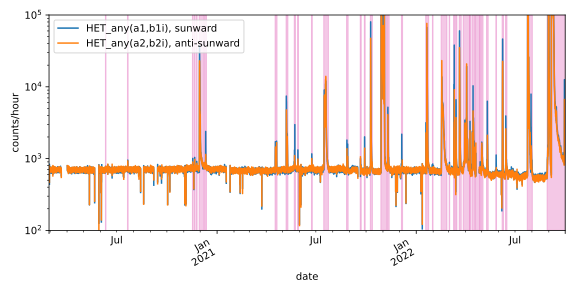
\includegraphics[width = \textwidth]{images/ACR/SOLO-lvl2-trriger-V2.png}
    \caption[The multiple detector counters of \ac{HET}]{Hourly count rate of the \ac{HET} multiple detector counters. The magenta-colored regions are the \ac{SEP} periods we identified.}
    \label{Fig:solo-lvl2}
\end{figure}



\begin{figure}
    \centering
    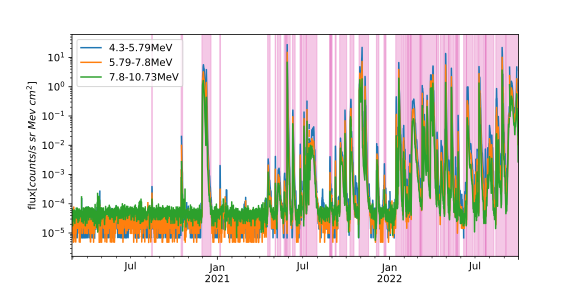
\includegraphics[width = 1\textwidth]{images/ACR/SOLO-EPHIN-l3i-log2+6-proton-6H-V2.png}
    \caption{The proton intensity profile observed by \ac{EPHIN}}{The proton flux measured by \ac{SOHO}/\ac{EPHIN} below 10 MeV. The data we used here are the level-3 proton data products \citep{kuehl2020JSWSC}. The magenta-colored regions are \acp{SEP} observed near Earth.}
    \label{Fig:SOHO_EPHIN_Proton_flux}
\end{figure}

\subsection*{Averaged over Carrington rotation}

As mentioned earlier, transient \acp{SEP}, long-term solar modulation, and periodic \ac{CIR} and \acs{SIR}\acused{SIR} affect the \ac{ACR} intensity. In the previous section, we identified and removed \ac{SEP} periods to obtain a slowly changing profile. In this section, we will further reduce the impact of recurring compressed regions by averaging the intensity profile over each Carrington rotation, as suggested by \citet{Rankin2021ApJ}. The Carrington rotations for \ac{SolO} are defined in the second panel from the top in Fig.~\ref{fig:SOLO_orbit_info} which depicts the change of \ac{SolO}'s Carrington longitude. 

%. Though that data point is from a Carrington rotation with a larger \ac{SEP} event, we have already removed the \ac{SEP} periods from the data. Besides, such an increase is even clearer in the higher energy channel (bottom panel). 

Fig.~\ref{fig:carrington_flux} displays the average helium flux from \ac{HET} (orange line) and \ac{EPHIN} (blue line). The red dashed lines indicate the variation in radial distance between \ac{SolO} and the Sun. The averaged flux decreases over time which is noteworthy. The measurements across all four channels are generally comparable, despite the anticipated radial gradient of approximately 25\%/au \citep{Rankin2021ApJ}.

However, we could still see some discrepancies that are worth noting. During the end of 2020 and the start of 2021, the \ac{HET} helium intensity is unusually high compared to that measured by \ac{EPHIN}. The discrepancies are up to 30 \% and are clearly seen in all four channels.

Furthermore, the bottom panel of Fig.~\ref{fig:carrington_flux} shows that before 2021, the intensities of 40 - 50 MeV/nuc helium from \ac{EPHIN} are statistically lower than that from \ac{HET}. After that, such a discrepancy gradually disappeared in this channel. Besides, such a discrepancy is unseen in the lower energy channels. Currently, the reasons for these discrepancies are unclear.

Fig.~\ref{fig:fluxvsdistance} illustrates the helium flux within the energy range of 10 - 20 MeV/nuc from \ac{HET}, as a function of the radial distance from 0.4 to 1 au. Averaged fluxes of four orbits are represented by distinct colors, as indicated in the legends. In addition, blue triangles that overlay solid circles suggest the time order of measurements. Notably, the intensity of helium at the last measurement point is about five times less than that at the beginning. Such a decrease is caused by the solar modulation. Removing this trend is discussed in the next section.

%Without carefully tackling this underlying baseline trend, we could not derive the radial gradient with a magnitude of $\sim$ 25\%/au.


% and the slight discrepancy in energy channels between \ac{HET} and \ac{EPHIN},

\begin{figure}
    \centering
    \includegraphics[width = 0.8\textwidth, height = 0.2\textheight]{images/ACR/seperate_mask_1-3_newSOHOSEPmask/Carrington_SOLO_11.1-19.4MeV_EPHIN_10.7-20.3MeV.png}
    \includegraphics[width = 0.8\textwidth,height = 0.2\textheight]{images/ACR/seperate_mask_1-3_newSOHOSEPmask/Carrington_SOLO_19.4-29.5MeV_EPHIN_20.3-28.0MeV.png}
    \includegraphics[width = 0.8\textwidth,height = 0.2\textheight]{images/ACR/seperate_mask_1-3_newSOHOSEPmask/Carrington_SOLO_29.5-41.2MeV_EPHIN_28.0-38.5MeV.png}
    \includegraphics[width = 0.8\textwidth,height = 0.2\textheight]{images/ACR/seperate_mask_1-3_newSOHOSEPmask/Carrington_SOLO_41.2-49.0MeV_EPHIN_38.5-53.0MeV.png}
    \caption[The averaged helium flux in four energy channels between 10 and 50 MeV/nuc]{The flux of \ac{SolO} (orange) and \ac{EPHIN} (blue) averaged over the Carrington rotation periods in the energy channels of 10 - 20 MeV/nuc, 20 - 30 MeV/nuc, 30 - 40 MeV/nuc and 40 - 50 MeV/nuc. The daily averaged \ac{HET} helium fluxes are also shown in different energy channels as light orange lines. Red dashed lines are the radial distance of \ac{SolO} to the sun.}
    \label{fig:carrington_flux}
\end{figure}

\begin{figure}
    \centering
    \includegraphics{images/ACR/SOLO-flux_only.png}
    \caption[10 - 20 MeV/nuc \ac{HET} helium flux vs the radial distance of \ac{SolO}]{The flux of 10 - 20 MeV/nuc helium from \ac{HET} changes with respect to the radial distance of \ac{SolO}. The data corresponding to different orbits are presented in distinct colors. The blue arrows indicate the time flow direction.}
    \label{fig:fluxvsdistance}  
\end{figure}


\section{Radial gradient of ACR helium}

Deriving the small radial gradient ( $\sim$ 25\%/au, \citet{Rankin2021ApJ}) from the substantially changed data is challenging, particularly when dealing with the five-fold decrease in helium intensity resulting from solar modulation.
To address this challenge and obtain the radial gradient, we detrend the \ac{HET} flux by using the \ac{EPHIN} flux as a baseline. We assume that the solar modulation is the same for both instruments. We first calculate the ratio of \ac{HET} and \ac{EPHIN} and then estimate the radial gradient of different energy \ac{ACR} helium using the definition in Eq.~\ref{eq:radial_gradient}.

We present the temporal variation of flux ratio between \ac{HET} and \ac{EPHIN} for four energy channels in the first and third rows of Fig.~\ref{fig:ratio_radialgradient}. The various colored regions represent periods of different orbits. The second and fourth rows illustrate the ratio in log scale as a function of the radial distance. Here, only the data points from of first three orbits are shown and fitted. That is because \acp{SEP} are the dominant particles in the fourth orbit. Hence, most of the data are removed, causing considerably higher uncertainties in the result. The colored dashed lines in the figure represent the fitting results obtained for different orbits. The shaded regions surrounding these lines are the corresponding 95\% confidence intervals,  indicating the uncertainty of the fitting results. The averaged radial gradients of the first three orbits are depicted as black dashed lines, indicating the overall trend between 2020 and 2022.
In addition, we have summarized the radial gradient of \ac{ACR} helium in different energy channels and for different orbits in Table~\ref{Tab:radialgradient_1}.

\begin{figure}[!htb]
    \centering
    \includegraphics[width =0.48\textwidth, height = 0.4\textheight]{images/ACR/seperate_mask_1-3_newSOHOSEPmask/ratio_time_radialgradient_10-20MeV.png}
    \includegraphics[width =0.48\textwidth, height = 0.4\textheight]{images/ACR/seperate_mask_1-3_newSOHOSEPmask/ratio_time_radialgradient_20-30MeV.png}
    \includegraphics[width =0.48\textwidth, height = 0.4\textheight]{images/ACR/seperate_mask_1-3_newSOHOSEPmask/ratio_time_radialgradient_30-40MeV.png}
    \includegraphics[width =0.48\textwidth, height = 0.4\textheight]{images/ACR/seperate_mask_1-3_newSOHOSEPmask/ratio_time_radialgradient_40-50MeV.png}
    \caption[Ratio of helium intensity between \ac{HET} and \ac{EPHIN} and helium radial grdient in different energy range]{Row 1 and 3: The temporal variation of the helium flux ratio between \ac{HET} and \ac{EPHIN} measurements (averaged over their own Carrington rotation and interpolated to calculate the ratio) for different energies; Row 2 and 4: Flux ratio vs radial gradients in the first three orbits, overlay by the log-linear fitting lines.} 
    \label{fig:ratio_radialgradient}
\end{figure}



\begin{figure}[!htb]
    \centering
    \includegraphics{images/ACR/Energydependent_normal_mask20230612.png}
    \caption[Energy dependency of the helium radial gradient]{The radial gradient of helium measured in the ecliptic plane at different energies. The values from \ac{HET} are given as orange diamonds with corresponding error bars. The multiple blue circles in the figure represent the gradient obtained from \ac{PSP} \citep{Rankin2021ApJ}.}
    \label{fig:comparison_SOLO_PSP}
\end{figure}

%  \TODO{New simulation and ask help from some one in Kiel, not now}.



\begin{table}[!htb]
    \centering
    \begin{tabular}{|c|c|c|c|c|c|}
        \hline
    Number of Orbit     & 1               & 2              & 3               & 4  & ave(1-3)\\
    \hline
                        &20200228 -      & 20201012-        & 20210602-    &  20211216-   &\\  
    Energy (MeV/nuc)    & 20201012        &  20210602       & 20211216      &  20220704  & \\

    \hline
    10 - 20 &  27 $\pm$ 9 & 38 $\pm$ 14 & 21 $\pm$ 19 & -25 $\pm$ 22 & 28$\pm$ 8\\
    \hline
    20 - 30 &  19 $\pm$ 9 & 28 $\pm$ 20 & 11 $\pm$ 15 & 33 $\pm$ 16 & 19$\pm$ 08\\
    \hline
    30 - 40 &  5 $\pm$ 14 & 12 $\pm$ 14 & 37 $\pm$ 21 & 8 $\pm$ 21 & 10$\pm$ 11\\
    \hline
    40 - 50 &  5 $\pm$ 9 & 27 $\pm$ 21 & 58 $\pm$ 19 & 20 $\pm$ 18 & 21$\pm$ 11\\
    \hline
    \end{tabular}
    \caption[Table of helium radial gradient]{Radial gradient of helium (\%/au) in different energy channels at different orbit between 2020 and 2022.}
    \label{Tab:radialgradient_1}
\end{table}
\subsection*{Radial gradient of helium vs energy}

Fig.~\ref{fig:comparison_SOLO_PSP} displays the energy dependence of the radial gradient of \ac{ACR} helium measured by \ac{PSP} and \ac{SolO}. 
Despite the large uncertainties, radial gradients of helium measured by \ac{SolO} averaged over the first three orbits are shown as orange diamonds. Except for helium in the energy range of 30 - 40 MeV/nuc, which has a lower average gradient of 10 $\pm$ 11 \% /au, we report radial gradients of 28$\pm$ 8 \%/au, 19$\pm$ 8 \%/au, and 21$\pm$ 11 \%/au for helium energies of 10 - 20 MeV/nuc, 20 - 30 MeV/nuc and 40 - 50 MeV/nuc respectively.
Such gradients are consistent with \ac{PSP}'s results within the uncertainties.
To compare with \ac{PSP} results derived by \citet{Rankin2021ApJ}, we replot helium radial gradients as the blue circles at their energy range. \ac{PSP} measurements are from 2018 to 2019 in the same solar activity minimum but earlier than \ac{SolO}. The averaged radial gradient of helium in the energy range of 4 - 45 MeVn/nuc is about 25$\pm$5 \%/au. 



\subsection*{The time variation of the radial gradient}

We also present the time variation of the helium radial gradients for different energy ranges from 10 - 50 MeV/nuc in Fig.~\ref{fig:radialgradient_time_variation}. The behaviors exhibited by the different energy channels are distinct, and the radial gradients show significant variations from 2020 to 2022, probably due to increased solar activity. Several intriguing features are observed in the time variation of the radial gradients, which are unexpected and hard to explain.

The peaks of radial gradients occur at different times for each energy channel. The highest radial gradient for the 10 - 20 Mev/nuc helium channel appears during the second orbit, while for the 30 - 50 Mev/nuc channels, the peaked gradients are observed in the subsequent orbit.

Furthermore, the sign of the radial gradient in the energy range of 10 - 20 MeV/nuc changes from positive to negative during the fourth orbit in 2022. This change could be attributed to the more considerable uncertainties introduced by \acp{SEP}. Because of the more frequently appeared \ac{SEP} in the fourth orbit, we might remove most of the data from \ac{EPHIN} measurements in one Carrington rotation, thus the remaning days' measurements are likely not representative for the whole Carrington rotation. Consequently, the Carrington averaged \ac{EPHIN} flux in the fourth orbit exhibit more fluctuations than the previous periods. 
An alternative explanation for the observed sign change in the radial gradient could be attributed to the complex magnetic field structures in the inner heliosphere governed by the Sun and solar activity. 
For instance, near the Sun, the radial components are overwhelmed by the transverse magnetic fluctuations \citep{Rankin2022ApJ} in the inner heliosphere below 1 au, causing a different transport environment than in the outer heliosphere.
On the other hand, with the Sun becoming more active than before, the large-scale \acs{HMF} might also be distorted by transient eruptions such as \acused{CME}\acp{CME}.

%From the averaged intensity we could find that the averaged helium flux from \ac{EPHIN} changed drastically between the consecutive carrington rotation. Unlike the similar change in the previous orbit, such change is due to the 

\begin{figure}[!htb]
    \centering
    \includegraphics[width = \textwidth, height = 0.3\textheight]{images/ACR/timevariation_normalmask_gradient.png}
    \caption[The time variation of the \ac{ACR} helium radial gradients]{The time variation of the \ac{ACR} helium radial gradients from 2020 to 2022. }
    \label{fig:radialgradient_time_variation}
\end{figure}



\section{ Summary and discussion}

We presented the \ac{ACR} helium in the energy range of 10 - 50MeV/nuc, measured by \ac{SolO}/\ac{HET} between Feb 2020 and Sep 2022. The first half of this time period was still the solar activity minimum at the end of solar cycle 24, characterized by minimal solar activity, while the second half witnessed an increasing number of \acp{SEP}.
Comparisons between the helium spectra obtained by \ac{HET}, \ac{EPHIN}, and \ac{ACE}/\ac{ACESIS} show general agreement. Furthermore, \ac{SolO} and \ac{ACE} exhibit consistent measurements of carbon, oxygen, and nitrogen.

By utilizing the \ac{EPHIN} measurements as a baseline, we derive the radial gradient of \ac{ACR} helium in the inner heliosphere. We reduce the effects of long-term solar modulation by dividing the intensity of  \ac{HET} by that of \ac{EPHIN} 
after we remove the interference by \acp{SEP} and the potential short-term variations due to \acp{CIR}.
We report that the radial gradients for helium energies of 10 - 20 MeV/nuc, 20 - 30 MeV/nuc, and 40 - 50 MeV/nuc are 28$\pm$ 8 \%/au, 19$\pm$ 8 \%/au, and 21$\pm$ 11 \%/au respectively. 
These results are consistent with gradients obtained by \ac{PSP} within the uncertainty. Interestingly, the averaged radial gradient in the energy range of 30 - 40 MeV/nuc is only half that in the other channels, about 10 $\pm$ 11 \%/au. Currently, those results are very preliminary, and more discussions are needed to improve the results and explain this feature.

The analysis above shows how challenging it is to derive the radial gradient of \ac{ACR} helium. In addition to the intensity decrease caused by the long-term solar modulation, the more problematic component is the remanent \acp{SEP} that could not be recognized from the time series of the proton flux from \ac{EPHIN} and the L2 trigger rate of \ac{HET}. Here we proposed additional methods to derive cleaner \ac{ACR} measurements.

The first method sets a threshold for the particle intensity that will be used to calculate the averaged flux. By doing so, the data points of intensity higher than the threshold will be filtered out. In practice, we chose the threshold of 95 \% of the sum of helium accumulated in one Carrington rotation. This method is under the assumption that the highest intensity particles are from \acp{SEP} that we could not identify. As a result, the radial gradients with this extra mask are consistent with the gradients we obtained above. We derive the gradients of 27 $\pm$ 7 \%/au , 16 $\pm$ 8 \%/au and 21$\pm$ 11 \%/au for helium energies of 10 - 20 MeV/nuc, 20 - 30 MeV/nuc and 40 - 50 MeV/nuc, respectively. 


Due to the high time resolution and limited \ac{FOV} of \ac{HET} data products, the count rates of helium measurements are discrete values and, most of the time, are zeros, as the data show. The distribution of the count rate should be described by a Poisson distribution with a parameter $\lambda$ equal to the mean values. 
The second method assumes that the \ac{ACR} background, that is unaffected by any modulation effects, has constant intensity during a certain period, for instance, one day. A mean value could represent the measurements of this background. However, when the background is interrupted by a short-time structures, regardless of whether it causes the flux to increase or decrease, the Poisson distribution with mean values as $\lambda$ can not model the count rate distribution. Note that this method is only applied to disentangle short-term changes. 
In practice, firstly, we calculate the mean value during one day. Secondly, we estimate the probability that the measurements follow a Poisson distribution with the $\lambda$ equals to the mean value.
By doing so, we obtain the same table as in Table \ref{Tab:radialgradient_1}, and the new results are given below in Table \ref{Tab:radialgradient_2}.
The averaged gradients over the first three orbits are 34 $\pm$ 8 , 22 $\pm$ 10, 19$\pm$ 11 for helium energies of 10 - 20 MeV/nuc, 20 - 30 MeV/nuc, and 40 - 50 MeV/nuc, respectively. 


We agree that some other methods could also be used to derive the radial gradient of \ac{ACR} helium in the future. For instance, we could use the median value rather than the mean value to represent the flux of the center Carrington rotation. The purpose of this method is that median values are less affected by outliers. Hence we could avoid the higher energy tails, if there are any, after we remove \acp{SEP} discussed before. Besides, we could also use the daily averaged flux rather than the mean value of a full Carrington rotation to calculate the ratio between \ac{HET} and \ac{EPHIN}. 


Furthermore, as discussed in \citet{Rankin2021ApJ}, the \ac{GCR}helium should also be considered in the energy range of 10 - 50 MeV/nuc. According to the spectra predicted from the simulation, the \ac{GCR} helium intensity increases with the energy increases before it peaks at few hundreds MeV. \citet{Rankin2021ApJ} found that after subtract the assumed \ac{GCR} intensity, the raidal gradient become larger. Therefore, we will also consider this correction in future work once we find a better way to estimate the varying \ac{GCR} helium intensity.

Here, we just present the result of our analysis for the radial gradient without giving any detailed explanations. Nevertheless, linking our current observations to the previous results and our present knowledge of the cosmic ray transport will significantly advance our understanding of the transport of \acp{ACR} in the inner heliosphere.
%Finally, we have averaged the helium intensity over a complete carringon rotation to remove the potential \ac{CIR} modulation effect. Howvever, e \ac{CIR} modulation might need to be further considered, 




\begin{table}[!htb]
    \centering

    \begin{tabular}{|c|c|c|c|c|c|}
    \hline
    Number of Orbit     & 1               & 2              & 3               & 4  & ave(1-3)\\
    \hline
                        &20200228 -      & 20201012-        & 20210602-    &  20211216-   &\\  
    Energy (MeV/nuc)    & 20201012        &  20210602       & 20211216      &  20220704  & \\
    \hline
    10 - 20 &  43 $\pm$ 10 & 21 $\pm$ 18 & 41 $\pm$ 13 & 40 $\pm$ 49  & 34 $\pm$ 8\\
    \hline
    20 - 30 &  34 $\pm$ 13 & 23 $\pm$ 19 & -9 $\pm$ 13 & -16 $\pm$ 28  & 22 $\pm$ 10\\
    \hline
    30 - 40 &  8 $\pm$ 15 & 19 $\pm$ 14 & 41 $\pm$ 22 & 10 $\pm$ 20 & 13 $\pm$ 12\\
    \hline
    40 - 50 &  15 $\pm$ 4 & 15 $\pm$ 24 & 55 $\pm$ 32 & 65 $\pm$ 33 & 19 $\pm$ 11\\
    \hline
    \end{tabular}
    \caption[Table of helium radial gradient with extra mask]{The radial gradient of helium (\%/au) in the same format as Tab.~\ref{Tab:radialgradient_1} but with extra mask to remove the potential short term variation. }
    \label{Tab:radialgradient_2}
\end{table}


%No matter how, those are the 

% The higher the energy , the deep the particle can penetrate into the heliosphere.

% The higher the solar modulation, the larger the radial gradient.

% General picture: the large the solar modulation, the strong the magnetic field, the large the radial gradient.

% The weak solar magnetic field could not effectively affect the transport of the high energy particles, or at least smaller compared to the lower energy particles.





%\input{chapters/pub04_xu2022}


\chapter{Summary and Outlook}
\label{chp:outlook}

The energetic particles in the heliosphere within the energy range of tens of Mev are of great importance, not only because of the abundant physics process they underly, but also due to their potential hazard to the human health, which is the requirement of space explorations.
Benefiting from two new instrumennts, \ac{LND} on board Chang'E-4 operating on the lunar surface and the \ac{HET} on board \ac{SolO} orbiting and approaching the Sun, and combined the multiple instrument observations,  we have a great oppurtunity to further our understand of these energetic particles.
Therefore, in this thesis, all three particle populations, \acp{SEP}, \acp{GCR} and \acp{ACR} are detailed investigated. The summary of the thesis and the outlooks is as follows.

%Amongest them, \ac{GCR}, ACR are from background and  SEP are the temporal increase. The particle full of different information of particle accerlerateion, injection, and propagtaion mechanismm.  
%Besides, the radiation hazard due those charge particles force us to study their time variation and spatial distribuions and the impact on the human body, which is the requirement of space explorations.


In the first publication presented in Chapter \ref{chp:LND_SEP}, we report the first \ac{SEP} event reaching the lunar far-side surface. This \ac{SEP}event have very weak intensity 
Our analysis consists both in-situ and remote-sensing data obtained from multiple instruments and perspectives. We first derived the proton integrated spectrum. Then we infered the release times of protons and electrons based on their clearly velocity dispersion. Based on results, We found an earlier injection of electrons than that of protons. 
Meanwhile, the solar eruption originating from a distant, solitary active region on the solar disk and a slowly moving \ac{CME} which is observed on the corongraph appear to be the most plausible source of these MeV energy particles in this event. We proposed potential transport mechanisms that could account for the traversal of protons and electrons within the lower coronal region and over the heliosphere, such as expanding \ac{CME}-driven shocks, irregular magnitic field lines, and even transport path diverging from the nominal Parker spiral field. Furthermore, in recent communications with Christina Cohen, the idea of the \ac{HCS} serving as the bridge between the active region and the \ac{L1} in this special case was brought up, even though the detailed transport mechanism remain unclear and need further investigation. Based on the above observations, we conclued that the protons and electrons behave differently in the release and transport process. Though we 

By analyzing various observations, we have provide plausibly solution in addressing the questions raised in the motivation section regarding the source of tens of MeV \acp{SEP} and their transport in the heliosphere. However, due to limited remote-sensing observation and single perspectives, we could not give a full picture of the event and determine the exactly roles that each potential factor play.  The recently study on the wide spread SEP from \citet{dresing202317, Kolhoff2021AA} indicates that the multiple observation and numberical simulation might help a lot on answering these questions.

In the second publications, the primary \ac{GCR} proton spectrum during 2019 - 2020 measured by \ac{LND} on the lunar surface is presented. This spectrum span the energy range from $\sim$ 10 to $\sim$ 400 MeV, including both the stopping particles and penetrating particles of \ac{LND}, though in the current stage, the uncertainty of penetrating data products is still higher than anticipated. The proton measurements from \acs{SOHO}/\acs{EPHIN} during the same periods in the energy range of 10 - 50 MeV are consistent with the \ac{LND} measurements. However, the GCR are higher than the previous solar activity minimum, reaching the historical record since the start of space age.  Moreover, we derived the intensities of 65 -76 MeV albedo protons on the lunar surface. The albedo protons are a subclass of the secondary particles which are generated after the interaction betweeen \ac{GCR} and lunar regolith. We found that the flux of albedo protons in this solar activity minimum is consistent with that in the previous solar acitivity minimum which was obtained by the \acs{LRO}/\acs{CRaTER} in 2009 - 2010. The study of albedo proton shed light into the lunar radiation environment and the seaching for the hydrogen on the lunar surface. 
%As a matter of fact, the \ac{LND} measurements can further define a albedo proton spectrum of several energy bins only if we have enough statistic. 
Meanwhile, the analysis of quite time spectra of protons,helium-4, helium-3, oxygen, carbon and iron from \citet{Mason-2021-SolOQuietTime} show how the ions spectra look like during the soalr minimum betweeen 0.5 - 1.0 au. The lower energy measurement are made by \acs{SIS} and the higher energy part are measured by \acs{HET}. These spectra is comprised of the GCR components, ACR components and lower energy turn-up spectrum which due to the impulsive \acp{SEP}. The ACR spectra is similar with that in the previous solar cycles. 

In the above two studies, we check the \ac{ACR}, \ac{GCR} in the heliosphere and on the lunar surface and secondary particles measured on the lunar surface.   We try answer the questions


%In particular, the super quiet time measurements show us how the particle spectra differ compare with normal quiet time. In the spectram GCR ACR and a turn-up spectrum 
%The helium turn-up 

%we did what, we found what, and the try to anwser which quesiton? Has you answer that? Any further expected from here?, what question are answer


In the last section of the thesis, we try to understand the distribution of the cosmic ray


The main topic of this thesis was to better understand the instrument and its new data around ten of Mev

The main goal is to look at the particles around ten of MeV using the new instrument and new time period

The data calibration and analysis are the main part of this thesis. 

Cross calibration of the new instruments:


In the end we try to give the answer to the instrumental question we ask in the motivation, how dose the new measurment look like, are they 


In the forth publication, we study the ACR measurements of Helium.

Let's re-visit the questions we 


We plan for the future study


\subsection*{Outlook}

By comparing the new measurement of \ac{SEP} and background cosmic ray, we conclude that new 



\subsubsection*{The relationship between SEPs and the radiation dose on the lunar surface}

LND and SOLO are two total new instruments.
LND have many many data and only few projects have been explored.
Below are several possilbe project that could be done with the LND data
1. Heavy ion spectra on the lunar surface. We only give the helium but the other heavy ion like carbon, nitrogen, and oxygen havent been explored. Data calibration need to be done( which is already finished in the past), 
2. Albedo particle more fine spectra
3. Connecting the observation dose and the model simulation - SEP and GCR
4. Discrepancy between LND and Crater.


\subsubsection*{The spatial gradient of ACRs and GCRs}
The spatial gradient of ACR oxygen and nitrogen


The spatial gradient of GCR helium


The spatial gradient of proton

% The goal of this thesis was to introduce observations at Mars as well as at \ac{SolO} into the framework of space weather observations in the inner heliosphere, and to gain a better understanding of the radial evolution of \acp{ICME}. This was achieved by making use of the \ac{FD} measurements available from the \ac{RAD} on Mars and from the \ac{HET} onboard \ac{SolO}.

% In the first two publications, shown in \autoref{chp:arrival_times}, we have assembled two catalogs of \ac{ICME} events that were associated with \acp{FD} at Mars, but were also observed from a second point --- either in situ during oppositions of Mars with Earth or one of the \acused{STEREO}\ac{STEREO} spacecraft \citep{Forstner-2018}, or remotely from the \ac{STEREO} \acp{HI} \citep{Forstner-2019}. These catalogs will serve as a useful resource for future studies and should be continued by including more recent events in the future.
% In the first article studying the events during opposition constellations, the cross-correlation function of the \ac{FD} measurements allowed us to directly derive the transit times from \SI{1}{\AU} to Mars for a statistical study. The comparison of these transit times with the in situ measured \ac{ICME} velocities at \SI{1}{\AU} allowed us to show for the first time that \acp{ICME} can continue to decelerate beyond the Earth orbit and that this effect depends on the \ac{ICME}'s velocity relative to the ambient solar wind. This confirms that theoretical models based on this relative velocity, such as the \ac{DBM}, are applicable even at larger distances from the Sun. The \ac{ICME} arrival times were also compared to the results of the WSA-ENLIL+Cone \ac{MHD} model, and we found that the mean deviations in the arrival time were comparable to those typically seen at other locations in the inner heliosphere.
% On the other hand, in the second publication, we used the \ac{FD} observations at Mars to validate the \ac{HI}-based arrival time estimations. The single-spacecraft reconstruction methods are not particularly precise, but their performance is in line with the results for other locations previously compiled by \citet{Moestl-2017-HelcatsHSO}. Stereoscopic triangulation methods may improve these results, but the loss of connection to the \ac{STEREO}-B spacecraft in 2014 (see \autoref{sec:stereohi}) and the focus of the \ac{HI} telescopes on the Earth-Sun line has prevented this for many Mars-directed events. In the future, data availability from the \ac{HI} instruments onboard \ac{SolO} and \ac{PSP} may make the application of such methods feasible again, and a recovery of \ac{STEREO}-B in the coming years as it comes back closer to Earth would of course be beneficial as well.

% With the study presented in \autoref{chp:fd_properties}, we shifted away from the mere analysis of arrival times to the investigation of other \ac{FD} properties. Based on the catalog assembled in \citet{Forstner-2019} as well as larger independent catalogs, we could reproduce a correlation of two \ac{FD} parameters with the \ac{RAD} measurements that was already known from previous studies at Earth, though the slope $A$ of this relation (not to be confused with the steepness of the \acp{FD} themselves) was different at Mars than at Earth. Through the consultation of analytical \ac{FD} models, we have found that this value $A$ is likely independent of the particle energies observed by the different instruments and that it rather serves as a measure of the increase of the \ac{ICME} or sheath structure's size between the two planets. This result was also supported by comparing the obtained ratio of $A$ values with theoretical first-order approximations of the expected magnitude of this broadening. In future studies, this hypothesis should be further validated by analyzing large samples of \acp{FD} at other heliospheric locations in the same way.

% In the two publications in \autoref{chp:september_event}, we have shown \ac{RAD} measurements of the severe space weather events observed on the surface of Mars in September 2017. These consisted of a \ac{SEP} event as well as the merging of multiple \acused{CME}\acp{CME} en route to Mars, which caused an enormous \ac{FD} following the \acp{SEP}. This serves as a case study of a complex space weather event seen at both Earth and Mars but should not be seen as a worst-case scenario, as the \ac{SEP} source did not have direct magnetic connection to Mars, and the increased radiation dose during the event was coincidentally almost compensated by the following large \ac{FD}.

% Finally, \autoref{chp:solo} introduced the measurement capabilities of the \ac{HET} onboard the \ac{SolO} mission, which launched in early 2020. While the measurement of \acp{FD} is not one of the main focuses of \ac{SolO} and instruments for the direct measurement of \ac{ICME} plasma and magnetic field are also available on the spacecraft, the first \ac{FD} observations we obtained clearly show the high resolution with which such events can be captured by \ac{HET}. The close alignment of \ac{SolO} and Earth during this event also makes it a suitable candidate for multispacecraft studies, and this was pursued in the publication with the application of the \acs{ForbMod} model to the \acp{FD} at \ac{SolO} and Earth. The reason for the disagreement of \acs{ForbMod} with the observations for this very slow \ac{CME} needs to be examined in more detail in the future, but our initial investigations presented in the article suggest that it may be due to interaction with the following \acl{SIR}.

% In a nutshell, this work, both in statistical and case-study form, has highlighted many different aspects of the propagation of \acp{ICME} in the inner heliosphere. Still, there are numerous open questions in this field, and future studies building upon our results will undoubtedly be important contributions to the better understanding of space weather events as well as the development of enhanced forecasting capabilities.


% ********************************************************************
% Backmatter
%*******************************************************
\newpage
\markboth{}{\thepage}
\cleardoublepage
\phantomsection
\addcontentsline{toc}{chapter}{Bibliography}

\printbibliography

\cleardoublepage
%*******************************************************
% Acknowledgements
%*******************************************************
\refstepcounter{dummy}
\pdfbookmark[0]{Acknowledgements}{Acknowledgements}
\chapter*{Acknowledgements}




At this point, I would like to thank everyone who supported me during the course of my PhD studies and my work on MSL/RAD, Chang'E 4 LND as well as Solar Orbiter EPD.

First of all, I am grateful to my supervisor Prof. Robert Wimmer-Schweingruber for the opportunity to work on these exciting projects, and his helpful advice. He also made it possible that these results could be published in scientific journals and presented at many international conferences. Sincere thanks also to Prof. Jingnan Guo, who supported my work since my bachelor's thesis, and who I wish all the best for her new position in China.

Furthermore, thanks to all my colleagues in the three mission teams for their continued support and helpful discussions, including Zigong Xu, Alexander Kollhoff, and my officemate Christoph Terasa for the productive and enjoyable collaboration, e.g. on low- and high-level software for the Solar Orbiter mission, which will hopefully facilitate the EPD data analysis in the Kiel team for years to come, and to the rest of the Extraterrestrial Physics group at Kiel University. I also thank the group of Manuela Temmer and Astrid Veronig at the University of Graz and Mateja Dumbović at Hvar Observatory with whom I worked in close collaboration for many of the Forbush decrease studies, and who I enjoyed meeting regularly at the conferences in Vienna, Hvar and San Francisco.

I additionally want to thank the bachelor and master students who supported my work during their Hiwi positions, Charlotte Büschel and Niklas Lundt, and three secondary school students, Joana Wanger, Lukas Abegg and Markus Arndt, who contributed to the data sets used in my studies during their internships in the ET group.

I would like to thank Anne Fischer as well as Hanna Giese and Knud Schröter for their very thorough proofreading of this thesis and valuable suggestions, and my parents Kristina and Michael and my brother Julius for their moral support. 

Last but not least, the data analysis presented in this thesis, the typesetting of the thesis itself and the generation of most of the figures were made possible by a number of open source software projects, including, but not limited to, the ones acknowledged below:

\begin{refsection}[software.bib]
	\nocite{*}
	\newrefcontext[sorting=none]
	\printbibliography[heading=none]
\end{refsection}

\cleardoublepage
\appendix
\include{chapters/Appendix_LNDsimulation}

\cleardoublepage
\include{chapters/Appendix_LNDNew_data_products}

\cleardoublepage
\chapter{List of publications}
\label{chp:Publicationlist}

This list shows all peer-reviewed publications that I have contributed to. Not all of these publications were included in this thesis, as they do not all fit into the logical flow of this thesis.\\

\noindent\pubcite{Xu2020ApJ}\\

\noindent\pubcite{Xu2022FrASS}\\

\noindent\pubcite{Wimmer2020SSRv}\\

\noindent\pubcite{Zhang2020SciAdv}\\

\noindent\pubcite{Forstner-2021-SolO}\\

\noindent\pubcite{Zhang2021ChJSS}\\

\noindent\pubcite{Mason-2021-SolOQuietTime}\\

\noindent\pubcite{Bucik2023AA}\\

\noindent\pubcite{Lario2022ApJ}\\

\noindent\pubcite{Allen2021AA_suprathermal}\\

\noindent\pubcite{Allen2021AA_venus}\\

\noindent\pubcite{Gomez2021AA}\\

\noindent\pubcite{Aran2021AA}\\

\noindent\pubcite{Mason2021AA}\\

\noindent\pubcite{Bucik2021AA}\\

\noindent\pubcite{Wimmer2021AA}\\

\noindent\pubcite{Kolhoff2021AA}\\

\cleardoublepage
%*******************************************************
% Declaration
%*******************************************************
\refstepcounter{dummy}
\pdfbookmark[0]{Eidesstattliche Erkl\"arung}{Eidesstattliche Erkl\"arung}
\chapter*{Eidesstattliche Erkl\"arung gemäss §9 der Promotionsordnung}
%\thispagestyle{empty}
\begin{otherlanguage}{ngerman}
Ich versichere an Eides statt, dass die vorliegende Abhandlung -- abgesehen von der Beratung durch meinen Betreuer und 
der angegebenen Literatur -- nach Inhalt und Form meine eigene Arbeit ist.

Ich versichere, dass die Arbeit weder ganz noch zum Teil schon einer anderen Stelle im Rahmen eines Prüfungsverfahrens vorgelegen hat.
%
Teile dieser Arbeit wurden bereits in Fachzeitschriften veröffentlicht und sind als solche gekennzeichnet.
%
Die Quellennachweise der jeweiligen Veröffentlichungen befinden sich ausschließlich in den zugehörigen 
Literaturverzeichnissen und werden nicht im Literaturverzeichnis dieser Abhandlung aufgeführt.

Ich versichere, dass die Arbeit unter Einhaltung der Regeln guter wissenschaftlicher Praxis der 
Deutschen Forschungsgemeinschaft entstanden ist.

Ich versichere, dass von mir noch kein frühererer Promotionsversuch unternommen wurde und mir auch kein akademischer 
Grad entzogen wurde.
\end{otherlanguage}


\bigskip
 
\noindent\textit{\myLocation, \myTime}

\smallskip

\begin{flushright}
    \begin{tabular}{m{8cm}}
        \\ \hline
        \centering\myName \\
    \end{tabular}
\end{flushright}

	
\end{document}